\documentclass[12pt]{report}
\usepackage[margin=1in]{geometry}
\usepackage[compact,raggedright]{titlesec}
\usepackage{setspace} % for single/doublespacing commands
\usepackage{graphicx} % including graphics
% \usepackage{sectsty} % sexy section headings
\usepackage{pdfpages} % including multipage pdfs
\usepackage[export]{adjustbox} % for graphic frames and center
\usepackage{siunitx}
\usepackage[numbered]{matlab-prettifier} % including matlab w/ syntax highlighting
\usepackage[T1]{fontenc} % prettier matlab font
\usepackage{xfrac} % more legible inline fractions (\sfrac)
\usepackage{lmodern} % font package for above
\usepackage{multicol} % multiple columns
\usepackage[justification=centering]{caption} % figure captions (force centering)
\usepackage{amsmath} % more math symbols and shit
\usepackage{enumitem} % add arguments for enumerate to change style
\usepackage[list=true]{subcaption} % subfigures with list of figure support
\usepackage{multirow}
\usepackage{mathtools}
\usepackage{booktabs}
\usepackage{color}
\usepackage{ulem}
\usepackage{blindtext}
\usepackage[numbers]{natbib}
\usepackage{contour}
\usepackage{tabularx}
\usepackage{circuitikz} % drawing fancy shit
\usepackage{cancel} % arrow and cross math cancel symbol
\usepackage{lineno}
\usepackage{framed}
\usepackage{amssymb} % special math symbols
\usepackage{listings}
\usepackage{array}
\usepackage{BOONDOX-cal} % fancy mathtype script
\usepackage{fancyhdr}
\usepackage{flowchart}
\usepackage{color, colortbl}
\usepackage{tocloft}
\usepackage{url}
\usepackage{etoolbox}
\usepackage[usestackEOL]{stackengine}
% \usepackage{hyperref}

\setlength{\parskip}{\baselineskip}%
\setlength{\parindent}{0pt}%

\setcounter{secnumdepth}{5}
\renewcommand{\bibname}{References}
\sisetup{output-exponent-marker=\ensuremath{\mathrm{e}}}
\newcommand{\PreserveBackslash}[1]{\let\temp=\\#1\let\\=\temp}
\newcolumntype{C}[1]{>{\PreserveBackslash\centering}p{#1}}
\newcolumntype{R}[1]{>{\PreserveBackslash\raggedleft}p{#1}}
\newcolumntype{L}[1]{>{\PreserveBackslash\raggedright}p{#1}}
\lstMakeShortInline[style=Matlab-editor]| % matlab inline escape character
\graphicspath{{images/}}
\renewcommand\thesection{\arabic{section}}
\renewcommand\labelitemi{---}
\lstset{numberstyle=\ttfamily\small\color{gray}}
\renewcommand\linenumberfont{\ttfamily\small\color{gray}}
\setlength\linenumbersep{6mm}
% \hbadness=99999  % or any number >=10000
\apptocmd{\sloppy}{\hbadness 10000\relax}{}{}
\usetikzlibrary{arrows,calc,patterns,angles,quotes}
% \usetikzlibrary{shapes.geometric}
% \usetikzlibrary{decorations.pathmorphing,decorations.pathreplacing} % for snakes!
% \usetikzlibrary{positioning, circuits.logic.US}
\newcommand{\Lag}{\mathcal{L}} % lagrangian L

\apptocmd{\sloppy}{\hbadness 10000\relax}{}{}
\setlength{\cftbeforetoctitleskip}{-2em}
% \allsectionsfont{\raggedright} % w/ secsty
\setlist[enumerate]{wide=0pt, widest=99,
                    leftmargin=\parindent,topsep=0pt,partopsep=0pt,
                    label=\thesubsubsection.\alph*,font=\itshape}

\newcommand{\hiddensubsection}[1]{
  \stepcounter{subsection}
  \subsection*{\arabic{section}.\arabic{subsection}\hspace{1em}{#1}}
}
\newcommand{\hiddenappsec}[1]{
  \stepcounter{section}
  \subsection*{\Alph{section}\hspace{1em}{#1}}
}
\newcommand{\hiddenappsub}[1]{
  \stepcounter{subsection}
  \subsection*{\Alph{section}.\Roman{subsection}\hspace{1em}{#1}}
}
\titlespacing{\section}{0pt}{2ex}{1ex}
\titlespacing{\subsection}{0pt}{1ex}{0ex}
\titlespacing{\subsubsection}{0pt}{0.5ex}{0ex}

% \looseness=-1 % for one-liners bleeding off into the next page

\begin{document}
\normalem
\begin{titlepage}
\flushleft
\doublespacing
\Large
\textsc{Test Document} \\
\normalsize
Trey Dufrene, Zack Johnson, David Orcutt, Alan Wallingford, Ryan Warner
\vfill
\center
\includegraphics[width=.45\textwidth]{logo}
\vfill
\flushleft
ME 407 \\
Preliminary Design of Robotic Systems \\
Embry-Riddle Aeronautical University \\
\vspace{2ex}
\begin{minipage}[c]{.5\textwidth}
\flushleft
\includegraphics[width=.95\textwidth]{erau}
\end{minipage}%
\begin{minipage}[c]{.5\textwidth}
\flushright
\includegraphics[width=.8\textwidth]{text}
\end{minipage}
\end{titlepage}

\pagenumbering{roman}
\begin{abstract}
The Manipulator for Educational Institutions with Open Source Integrated Systems (MEIOSIS) aims to increase the accessibility of robotics to secondary educational institutions and hobbyists. Accordantly, the manipulator is 3D printed in PLA with aluminum tube supports and costs the end-user less than \$1000. The manipulator has six links and a base. The base houses a Raspberry Pi 3B and power supply. The Raspberry Pi controls seven Dynamixel smart servos with position feedback and proportional derivative control. Six MX-12W servos actuate six rotational joints, while one AX-12A servo actuates the removable end-effector. They provide the manipulator a position repeatability within 2mm of the previous pose. The manipulator can draw as well as perform pick and place operations within its dexterous workspace which is a hemispherical sub-shell of the reachable workspace of 280 mm thickness. The manipulator’s operation is controlled by open-source software.
\end{abstract}
% {\tableofcontents\let\clearpage\relax\listoffigures\let\clearpage\relax}
{\tableofcontents\clearpage\listoffigures\clearpage\listoftables}
\clearpage
\newpage
\section*{List Of Acronyms and Abbreviations}
\begin{tabular}{rcl}
  FK &:& Forward Kinematics \\
  IK &:& Inverse Kinematics  \\
  PD &:& Proportional Derivative \\
  % $k$~:& Spring constant \\
  % $h_{b}$~:& Distance to bar ($G$) from datum \\
  % $F_s$~:& Force onto bar due to spring\\
\end{tabular}

\section*{Notation}\vspace{-\baselineskip}
\renewcommand{\arraystretch}{2.25}
\begin{tabular}{rcl}
\large%
\(
{}^{\text{\scriptsize Frame}}_{\text{\scriptsize From}}~{r}~_{\text{\scriptsize To}}
\)\normalsize &:& Direction Vectors\\
\(
{}^{\text{\scriptsize From}}~{T}~_{\text{\scriptsize To}}
\)\normalsize &:& Direction Cosine (Transformation) Matrices \\
\(c_{\theta_{nm}}\)&:& \( \cos(\theta_n + \theta_m)\)\\
\(s_{\theta_{nm}}\)&:& \( \sin(\theta_n + \theta_m)\) \\
\end{tabular}
\renewcommand{\arraystretch}{1}
\newpage
\pagenumbering{arabic}
\section{Introduction}
Robotics is a rapidly growing field, yet numerous potential innovators for the discipline are never exposed to it. While many industrial style manipulators are available for commercial applications, their cost is so high that they are not practical for educational purposes. With the intention of making robotics education more accessible to classrooms, the Manipulator for Educational Institutions with Open Source Integrated Systems (MEIOSIS) aims to provide robotics classes with an accurate and precise manipulator for cost lower than traditional manipulators. MEIOSIS is designed to be 3D printed by the end-user to increase accessibility of the manipulator and will be modifiable to help create an increased understanding of robotics. The following document details the entirety of the design process, from conceptual design and definition of requirements to final implementation and testing.

\section{Conceptual Design}
The terminator T-2000 is a science-fiction spectacle of a robot -- until you see the price. Channeling the inspiration many high school students may have for robotics, MEIOSIS robotics aims to provide an affordable manipulator to educators and enthusiasts. MEIOSIS uses primarily 3-D printed components and easily accessible materials. Among these materials are a Raspberry PI, smart servos and metal tubing. These features create an open-source manipulator accessible to the public to further robotics education.
\hiddensubsection{Physical System Overview}
The physical design of the robotic manipulator will be shown through Figures \emph{\ref{fig:overall}, \ref{fig:base}, \ref{fig:link1},} and \emph{\ref{fig:link2}}.

\begin{figure}[htp]
  \centering
  \includegraphics[frame, width=.75\textwidth]{overall_render}
  \caption{Overall System Conceptual Design }
  \label{fig:overall}
\end{figure}

The colored links in \emph{Figure \ref{fig:overall}} distinguish the different joints and links of the manipulator. The overall reach of the robot will be 582.5 mm. This length was chosen to decrease material cost and weight while still satisfying requirement 2.1.2 and 2.1.5, allowing the manipulating to pick and place objects to perform basic tasks. The base of the robot will be made to contain the Raspberry Pi and other electrical components.
\newpage
\subsubsection{Base}
The base of the manipulator will house several of the electronic components, such as the computational system, power supply, and motor controller. A cross section of the base can be seen in \emph{Figure \ref{fig:base}}.
\begin{figure}[htp]
  \centering
  \includegraphics[frame, width=.75\textwidth]{base_callouts}
  \caption{Manipulator Base with Call-outs}
  \label{fig:base}
\end{figure}

From \emph{Figure \ref{fig:base}},
\begin{enumerate}[label=\alph*.]
  \item \emph{Base Supports:}
  The base supports are located at each corner of the base and will allow the base of the manipulator to be securely attached to a variety of surfaces with either standard bolt/fastener hardware or suction cups.
  \item \emph{Computational System:}
  The computational system will be a Raspberry Pi; it will be housed in the base, which allows the Raspberry Pi to be more easily accessible. The primary reason for this system being chosen is to fulfill the budget requirement, 2.1.1. The Raspberry Pi will compute the manipulator's kinematics and command the motors accordingly.
  \item \emph{Airflow Cutouts:}
  The side of the base will have cutouts to allow for airflow through the base; since the power supply is housed inside of the base as well as the computational system, the temperature must be regulated to prevent overheating.
  \item \emph{Power Supply:}
  The power supply will be housed in the base as well; this allows the power supply to be more accessible and therefore more modifiable, so the end-user can easily expand the system to fulfill their needs.
\end{enumerate}
\newpage
\subsubsection{Links}
\emph{Figure \ref{fig:link1}} is an image of the robot that shows the links and their key features.\\
\begin{figure}[htp]
  \centering
  \includegraphics[frame,width=.63\textwidth]{link_callouts}
  \caption{Drawing Showing Key Features of Design}
  \label{fig:link1}
\end{figure} \\
\emph{Figure \ref{fig:link1}} highlights a few of the key features of our design. Call-out a shows the connection point for the end effector. The mountings are the standard used by the Sawyer manipulator. This may be adjusted to accommodate lower cost, more accessible end effectors. Call-out (b) shows the differential gearbox that will be used in the manipulator’s wrist, saving space and weight. The manipulator will have aluminum tubing as support in the links (c) and will be attached to the 3D printed portion of the robot using clamp joints (d) tightened by screws.

\emph{Figure \ref{fig:link2}} is an image of the cross section of link 2 for the manipulator.
\begin{figure}[htp]
  \centering
  \includegraphics[frame,width=.35\textwidth]{link_cross_section}
  \caption{Drawing Showing Link Cross Section}
  \label{fig:link2}
\end{figure}

The cross section seen in \emph{Figure \ref{fig:link2}} shows the internal design for links two and three. It features two clamps that hold a hollow aluminum bar in place (a) and allows for gaps between the aluminum tube and the 3D printed call-out (b). The proper length will be dictated by the 3D printed guides lining up at call-out (c). This allows for imprecision in the manufacturing of the aluminum tube.

\hiddensubsection{System Functions}
The system can be divided into two subsystems: the electrical and software systems. The electrical subsystem includes the wiring and hardware computational components, power system, actuators with drivers, and sensors. The software subsystem includes the algorithm for the computational system.
\hiddensubsection{Electrical}
\emph{Figure \ref{fig:eblock}} is the block diagram for the electrical system of the manipulator.

\begin{figure}[htp]
  \centering
  \includegraphics[width=.55\textwidth]{eblock}
  \caption{Electrical System Block Diagram}
  \label{fig:eblock}
\end{figure}

\emph{Figure \ref{fig:eblock}} shows that the electrical systems of the manipulator will be relatively simple. Power is supplied by the 120V AC from standard wall outlets. A power supply will adapt the AC voltage to the required voltages for each component. One component is the Raspberry Pi, which will perform calculations for motor control (described below in software). It will send signals to the DC motor driver and the five smart servos. The smart servos have an on-board controller, so no feedback will be necessary. However, the first joint, between the base and the first link, will be actuated by a DC motor with an encoder to minimize cost.

\hiddensubsection{Software}
\emph{Figure \ref{fig:sblock}} shows the software flowchart for the system.
\begin{figure}[ht]
  \centering
  \includegraphics[width=.85\textwidth]{sblock}
  \caption{Software Flowchart}
  \label{fig:sblock}
\end{figure}

Similar to the electrical system, the software is also simple. \emph{Figure \ref{fig:sblock}} shows that the software will receive the desired pose or poses the user would like the manipulator to reach. Then the Raspberry Pi will use inverse kinematics to calculate the necessary joint angles. The wave-forms/desired angles will be sent to the respective drivers/motors, and positional information will be sent back to the Raspberry Pi to adjust the DC motor angle. When the motors have reached their desired pose, the Raspberry Pi will actuate the end effector if it is specified by the user. The system will then check to see if there are any more poses to reach and either repeat the motor control section given the desired angles of the new pose or end program if the last pose has been reached.

\newpage
\section{Specifications}
% \hiddensubsection{Introduction}
\label{sec:intro}
With the intention of making robotics education more accessible, The Manipulator for Educational Institutions with Open Source Integrated Systems (MEIOSIS) intends to provide high school educators and robot enthusiasts with a low cost manipulator. The system should be usable by novice students. It should also be modifiable to create a sustainably increased understanding of robotics. While MEIOSIS may not fully emulate industrial manipulators, it aims to provide more students with access to robotics education. \\
\begin{figure}[htp]
  \centering
  \includegraphics[frame,width=.75\textwidth]{model}
  \caption{Overview of Physical System}
  \label{fig:model}
\end{figure}
\newline
The design seen in \emph{Figure \ref{fig:model}} is based on our conceptual design. It features four links and six joints for rotation and will be referenced throughout this document. The base of the manipulator and end-effector can also be seen in the figure.
\hiddensubsection{Design Requirements}
The specifications of the system are strictly based on the requirements defined previously. The requirements are divided into two primary categories, hardware and software.
\vspace{-\baselineskip}
\hiddensubsection{Hardware}
The following requirements and specifications are hardware specific and dictate the physical constaints the system must adhere to.
\vspace{-\baselineskip}
\subsubsection{The system shall cost the end-user no more than \$1000.}
\begin{enumerate}
  \item \textit{The cost for the MEIOSIS team to develop the manipulator shall cost no more than \$800.}
\end{enumerate}

\subsubsection{The system shall be fully dexterous without being kinematically redundant.}
\begin{enumerate}
\item \textit{The system shall consist of six rotational joints connected by four links. The last three joints will create a spherical wrist.}
\end{enumerate}
As defined \cite{robo}, “A manipulator having more than six DOF is referred to as a kinematically redundant manipulator (5).” A manipulator with less than six degrees of freedom will not be fully dexterous within it's workspace. \emph{Figure \ref{fig:zero}} (see subsection \ref{sec:zero}, p. \pageref{fig:zero}) shows a six degree-of-freedom rotary manipulator with it's coordinate frames in zeroed positions. The joint and link locations are seen in \emph{Figure \ref{fig:model}} (see section \ref{sec:intro}, p. \pageref{sec:intro}).
\begin{enumerate}[resume]
\item \textit{The system shall have no link offsets.}
\end{enumerate}
Link offsets as seen in \emph{Figure \ref{fig:offset}} are commonly used to avoid singularities. However, having a link offset prevents the manipulator's dexterous workspace from being a complete hemispherical shell.

\begin{figure}[htp]
  \centering
  \includegraphics[width=.25\textwidth]{offset}
  \caption[Elbow Manipulator Configuration with Link Offset]{Elbow Manipulator Configuration with Link Offset \cite{robo}}
  \label{fig:offset}
\end{figure}
As shown in \emph{Figure \ref{fig:offset}}, the line directly above the first joint of the manipulator is offset such that the axes of the other joints are unable to become collinear with the base axis; this prevents singularity but causes a void in the detxterous workspace.
\subsubsection{The system end effector shall maintain a positional accuracy magnitude of \(\pm 1\) mm and an orientation accuracy of \(\pm 5^{\circ}\) eigen angle from the base frame.}
To ensure that the robot has educational value, the accuracy must be defined so that any desired positions and movements are achieved.
\begin{enumerate}
  \item \textit{The system shall accommodate a process in which the end user can calibrate the end effector position and orientation to within 0.5 mm and 1 degree of the manipulator’s precision.}
\end{enumerate}
The addition of a calibration process allows the removal of any systematic errors, such as drift. The theoretical limit of the calibration process is the difference between the precision and accuracy metrics of the system.
\subsubsection{The system end effector shall maintain a pose repeatability magnitude between 0.1—1.5 mm for the position and \(\pm 4^{\circ}\) eigen angle from the base frame for the orientation.}
\begin{enumerate}
  \item \textit{Joint one and two of the system shall possess an angle error of no more than .025 degrees.}
\end{enumerate}
Being that joint one and two are the first two rotational elements in the system, their error will propagate the most to the end effector's position.
\begin{enumerate}[resume]
  \item \textit{Joint three of the system shall possess an angle error of no more than .03 degrees.}
\end{enumerate}
Since joint three is closer to the end effector it's error will not propagate as severely throughout the system.
\begin{enumerate}[resume]
  \item \textit{Joints four, five, and six shall possess an angle error of no more than .29 degrees.}
\end{enumerate}
The spherical wrist is the closest to the end effector's final position and therefore has the least error propagation.

\subsubsection{The system’s reachable workspace shall be a hemisphere with a radius of 300-700 mm.}
This workspace will provide enough movement to manipulate objects in order to perform basic tasks.
\begin{enumerate}
  \item \textit{The length of link one, two, three, four, and the wrist shall be 220.8 mm, 250 mm, 200 mm, 80 mm, and 52.5 mm respectively.}
\end{enumerate}
  This results in a total height of 220.8 mm with a total reach of 582.5 mm in the zeroed configuration as shown in the configuration represented in \emph{Figure \ref{fig:zero}}.

\subsubsection{The system’s dexterous workspace shall contain a hemispherical shell within the reachable workspace with a thickness of 280 mm.}\label{sec:zero}
This workspace will provide enough movement to manipulate objects in order to perform basic tasks. 280mm is slightly greater than the length of letter paper.
\begin{enumerate}
  \item \textit{The rotational limit of joint one, two, three, four, five, and six shall be \(\pm180^{\circ}\), \(-9.7^{\circ}\) to \(177.5^{\circ}\), \(-150.6^{\circ}\) to \(-19.3^{\circ}\), \(\pm180^{\circ}\), \(-180^{\circ}\) to \(-1.6^{\circ}\), and \(\pm180^{\circ}\) respectively.}
\end{enumerate}
The angles stated are with respect to the kinematic model shown in \emph{Figure \ref{fig:zero}}. To be fully dexterous within our 280 mm dexterous workspace the manipulator must have the joint angles specified above. The joint limitations were calculated by iteratively verifying the orientation about every point within the quarter hemisphere cross section seen in \emph{Figure \ref{fig:dex}} (see Appendix, p. \pageref{sec:app}).
  \begin{figure}[htp]
    \centering
    \includegraphics[width=.75\textwidth]{zero}
    \caption[Kinematic Model Representing Zeroed Configuration]{Kinematic Model Representing Zeroed Configuration \cite{robo}}
    \label{fig:zero}
  \end{figure}
\subsubsection{The system shall have a removable end effector capable of picking and placing a low-odor chisel tip Expo dry erase marker.}
This creates a robot capable of performing a variety of basic tasks, which enhances its educational value.
\begin{enumerate}
  \item \textit{The system shall use a parallel gripper that can close to 18mm.}
\end{enumerate}
The diameter of a low-odor chisel tip Expo dry erase marker is approximately 18 mm.
\begin{enumerate}[resume]
  \item \textit{The end effector shall attach to the manipulator using screws configured in a pattern that can accommodate a Dynamixel AX-12A servo.}
\end{enumerate}
It is expected that a majority of end effector styles will have to accommodate for a servo to facilitate actuation, therefore a pattern was chosen to standardize the mounting.


\subsubsection{The system shall be able to write with a low-odor chisel tip Expo dry erase marker.}
\begin{enumerate}
  \item \textit{The end effector shall be able to support 0.004 Newton meter moments about the axes normal to its gripping surfaces.}
\end{enumerate}
  The coefficient of friction between the Expo marker and paper can be approximated and given the weight of an Expo marker the approximate grip strength of the end effector can be calculated.
\hiddensubsection{Software}
The following requirements and specifications are software specific and determine the attributes of the operating system.
\subsubsection{The system shall be open source.}
This will create an easily obtainable, low cost method of distributing the system’s source code, which may be modified for personal use.
\begin{enumerate}
  \item \textit{The software shall be hosted publicly on an online repository and maintain an MIT license for distribution.}
\end{enumerate}
  This allows the end-user to freely download and modify the code without licensing. The MIT license disregards any legal obligation to code upkeep and documentation by the original author.

\subsubsection{The system shall be capable of operating given only desired end effector cartesian coordinates specified with respect to the base frame.}
\begin{enumerate}
  \item \textit{The system shall have a user interface capable of accepting the end-effector’s desired cartesian position and Euler angle orientation as a six element row vector.}
\end{enumerate}
  The system software interface facilitates an untrained user to operate without the advanced knoledge of the system's kinematics.
\begin{enumerate}[resume]
  \item \textit{The system shall be capable of performing floating point arithmetic.}
\end{enumerate}
The solution for the inverse kinematics requires the ability to perform high level arithmetic with little error.

\newpage
\section{Preliminary and Detailed Design}
\section{Electrical System}
\section{Mechanical System}
\subsection*{Description of Mechanical Design}
One of the main differences between the conceptual mechanical design and the final design is the inclusion of 3D-printed harmonic gearboxes. The previous designs utilized a combination of standard spur gears and timing belts. It was determined that neither of these options provided the necessary precision without also introducing backlash into the system, which is nearly impossible to correct for with our feedback configuration. The solution was to design and implement a harmonic drive system. The harmonic gearbox locations are shown below in Figure \ref{fig:HarmonicGearboxLocations}.

\begin{figure}[htp]
  \centering
  \includegraphics[width=.65\textwidth,frame]{HarmonicGearboxLocations}
  \caption{Harmonic Gearbox Locations}
  \label{fig:HarmonicGearboxLocations}
\end{figure}

As seen in Figure \ref{fig:HarmonicGearboxLocations}, each joint only requires a single actuator, which is a configuration not seen in the previous design. This is possible because harmonic drives allow for very high gear ratios with minimal backlash. The first prototype harmonic drive was provided by a posting on Thingiverse. This design was meant to be driven by a stepper motor and provided a gear ratio of 39:1. However, the gearboxes implemented in the manipulator need to be driven by a smart servo. Because the smart servo cannot drive as fast as a stepper motor, the ratio of 39:1 resulted in joint movement that was extremely slow. Additionally, given the link lengths and precision of the servos, only a gear ratio of 20:1 was necessary to meet the precision requirements of the system. For these reasons, a second harmonic drive was designed to provide the proper gear ratio of 20:1. Figure \ref{fig:ExplodedViewoftheHarmonicGearbox} provides an exploded view of the main structural components of the newest harmonic drive.

\begin{figure}[htp]
  \centering
  \includegraphics[width=.65\textwidth,frame]{ExplodedViewoftheHarmonicGearbox}
  \caption{Exploded View of the Harmonic Gearbox}
  \label{fig:ExplodedViewoftheHarmonicGearbox}
\end{figure}

As seen in Figure \ref{fig:ExplodedViewoftheHarmonicGearbox}, the basic harmonic drive design features an outer housing, a stiff output shaft, a flexible gear, and a bearing holder assembly. When fully assembled, the bearing holder sits on the inside of the flexible gear. As the servo drives the inner bearing holder, a continuous meshing of teeth occurs between the flexible gear and the set of teeth that are built into the outer housing. Because the inner set of teeth has two less teeth than the outer set (the inside has 40 while the outside has 42), the inner gear will move forward by two teeth per rotation of the bearing holder. This results in 1/20th of a rotation of the flexible gear per full rotation of the bearing holder. With the output shaft being attached to the flexible gear, the whole harmonic drive provides a ratio of 20:1.

\subsubsection*{Equations of Motion}
Given robot dynamics described by \(H(\gamma) \ddot{\gamma}+d(\gamma, \dot{\gamma})+G(\gamma)=F_{\gamma},\) the equations of motion for
the manipulator can be determined. Solving this equation for the acceleration, \(\ddot{\gamma}\), gives:
\begin{equation}
  \ddot{\gamma}=H(\gamma)^{-1}\left(F_{\gamma}-d(\gamma, \dot{\gamma})-G(\gamma)\right)
  \label{eq:eoms}
\end{equation}
Where $H$ is the system mass matrix, $F_{\gamma}$ is the vector of generalized forces, $d$ is the vector of centripital and coriolis effects, and $G$ is gravitational effects.
\[
  \renewcommand{\arraystretch}{1.5}
  H(\gamma) = \sum_B^N J_B(\gamma)^T
  \begin{bmatrix}
    ^B_BJ & \mathring{S}(^B_B\Gamma) ^IT_B^T\\
    ^IT_B\mathring{S}(^B_B\Gamma)^T & m_BI
  \end{bmatrix}
  J_B(\gamma)~,\quad
  ^B_B\Gamma = ^B_Br_{cm}m_b~,\quad \mathring{S}(\omega)r=(\omega\times r)
\]
\[
  \renewcommand{\arraystretch}{1.5}
  d(\gamma,\dot{\gamma}) = \sum_B^N J_B(\gamma)^T
  \begin{bmatrix}
    ^B_BJ & \mathring{S}(^B_B\Gamma) ^IT_B^T\\
    ^IT_B\mathring{S}(^B_B\Gamma)^T & m_BI
  \end{bmatrix}
  \dot{J}_B(\gamma,\dot{\gamma})\dot{\gamma}+J_B(\gamma)^T
  \begin{bmatrix}
    ^B_B\omega_I \times ^B_BJ ^B_B\omega_I \\
    ^IT_B\left(^B_B\omega_I\times(^B_B\omega_I\times^B_B\Gamma)\right)
  \end{bmatrix}
\]
\[
G(\gamma) = \left(\frac{\partial U(^Ir(\gamma))}{\partial\gamma}\right)^T~,\quad U_B = \begin{bmatrix} 0 & 0 & g\end{bmatrix}\left(^I_Br_Bm_B + ^IT_B{}_B^B\Gamma\right)
\]
Where $J_B$ is the jacobian of the body, $\Gamma$ is the vector of first mass moments, $m_B$ is the mass of the body, and $^B_B\omega_I$ is the rotational velocity of the body relative to the inertial frame.

\subsubsection*{Actuator Dynamics}
Given robot dynamics described by \(H(\gamma)\ddot{\gamma} + n(\gamma,\dot{\gamma}) = \tau\), the torque, $\tau$, provided by the servo motors is necessary to solve the closed loop dynamics of the system. Assuming the servo is driven by a D.C. motor with proportional derivative control,
\begin{equation}
  \tau_a = Ki_a = J_a\ddot{\theta}_a + b_a\dot{\theta}_a + \tau_L
  \label{eq:motor}
\end{equation}
Where $\tau_a$ is the actuator torque, $K$ is the back-EMF constant, $i_a$ is the motor current, $J_a$ is the armature inertia, $\theta_a,~\dot{\theta}_a,\ddot{\theta}_a$ is the motor position and it's first and second time derivatives respectively, $b_a$ is the viscous friction coefficient, and $\tau_L$ is the torque available for the actuator to do work. The basic equation for a motor is known to be:
\begin{equation}
  V_a = i_aR_a + K\dot{\theta}_a
  \label{eq:va}
\end{equation}
Where $V_a$ is the voltage applied to the actuator and $R_a$ is the armature resistance. Given a gearbox with $\sfrac{\text{in}}{\text{out}}$ ratio $N$ and efficiency $\eta$,
\begin{center}
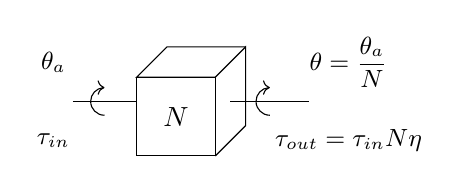
\begin{tikzpicture}
\pgfmathsetmacro{\cubex}{1}
\pgfmathsetmacro{\cubey}{1}
\pgfmathsetmacro{\cubez}{1}
\draw (0,0,0) -- ++(-\cubex,0,0) -- ++(0,-\cubey,0) -- ++(\cubex,0,0) -- cycle;
\draw (0,0,0) -- ++(0,0,-\cubez) -- ++(0,-\cubey,0) -- ++(0,0,\cubez);
\draw (0,0,0) -- ++(-\cubex,0,0) -- ++(0,0,-\cubez) -- ++(\cubex,0,0);
\draw (-2,-.5,-.5) -- ++(.8,0,0) node(a)[midway,above]{} node(b)[midway]{} node(c)[midway,below]{};
\pic [draw,angle radius=5,<-] {angle = a--b--c};
\node at (-2.25,0,-.5) {\small $\theta_a$};
\node at (-2.25,-1,-.5) {\small $\tau_{in}$};
\draw (0,-.5,-.5) -- ++(1,0,0);
\draw (0,-.5,-.5) -- ++(1,0,0) node(a1)[midway,above]{} node(b1)[midway]{} node(c1)[midway,below]{};
\pic [draw,angle radius=5,<-] {angle = a1--b1--c1};
\node at (1.5,0,-.5) {\small $\theta=\dfrac{\theta_a}{N}$};
\node at (1.5,-1,-.5) {\small $\tau_{out}=\tau_{in}N\eta$};
\node at (-.5,-.5,0) {$N$};
\end{tikzpicture}
\end{center}

The motor equation (\ref{eq:motor}) can be expressed in the output coordinates:
\[
Ki_a = J_aN\ddot{\theta} + b_aN\dot{\theta} + \frac{\tau}{N\eta}
\]
Substituing into equation (\ref{eq:va}) and solving for $i_a$:
\[
  i_a = \frac{J_aN}{K}\ddot{\theta} + b_aN\dot{\theta} + \frac{\tau}{N\eta}
\]
\begin{equation}
  V_a = \frac{R_aJ_aN}{K}\ddot{\theta} + \frac{R_ab_aN}{K}\dot{\theta} + \frac{R_a}{KN\eta}\tau + KN\dot{\theta}
  \label{eq:newva}
\end{equation}
Assuming PD control, \(V_a = K_p(\theta-\theta_d) + K_d\dot{\theta}\), where $\theta_d$ is the desired orientation of the actuator, the following solution is found by setting the PD solution equal to (\ref{eq:newva}). After collecting like terms:

\begin{equation}
  \frac{R_aJ_aN}{K}\ddot{\theta} + \left( \frac{R_aJ_aN}{K} - K_d + KN \right)\dot{\theta} - K_p\theta = -K_p\theta_d - \frac{R_a}{KN\eta}\tau
  \label{eq:end1}
\end{equation}
% \newpage
The following parameters of the system can be obtained by applying a step input to the system with $\tau=0$ and measuring the characteristics of it's response. Denoting $\zeta$ as the damping ratio and $\omega_n$ as the natural frequency of the system,
\[
  \text{\% Overshoot} = \left( \frac{\theta_{max} - \theta_{ss}}{\theta_{ss}} \right) \times 100~,\quad \zeta = \frac{-\ln(\sfrac{\%\text{OS}}{100})}{\sqrt{\pi^2 + \ln^2(\sfrac{\%\text{OS}}{100})}}~,\quad \omega_n = \frac{\pi}{T_p\sqrt{1-\zeta^2}}
\]

Given $\theta_{max},~\theta_{ss},$ and $T_p$ as measured parameters of the system's max output, steady state, and time to peak, respectively.

Refactoring equation (\ref{eq:end1}) and equating with the general solution for a second order system given by $\ddot{\theta} + 2\zeta\omega_n\dot{\theta} + \omega_n^2\theta = \omega_n^2\theta_d$, the following solutions are found:

\begin{minipage}[c]{.5\textwidth}
\begin{equation}
  2\zeta\omega_n = \frac{b_a}{J_a} - \frac{KK_d}{R_aJ_aN} + \frac{K^2}{R_aJ_a}
  \label{eq:one}
\end{equation}
\end{minipage}%
\begin{minipage}[c]{.5\textwidth}
\begin{equation}
  \omega_n^2 = \frac{-KK_p}{R_aJ_aN}
  \label{eq:two}
\end{equation}
\end{minipage}

Performing a similar experiment as previously described, except with a known inertial load $\tau = J_m\ddot{\theta}$, the following parameters can be found:
\[
  \alpha_m \equiv 2\zeta\omega_n = \frac{R_ab_aN^2\eta-KK_dN\eta+K^2N^2\eta}{R_aJ_aN^2\eta+R_aJ_m}~,\quad
  \beta_m \equiv \omega_n =-\frac{KK_pN\eta}{R_aJ_aN^2\eta+R_aJ_m}
\]

\begin{equation}
\begin{bmatrix}
  1 & -(\alpha_1J_1+\beta_1J_1) \\
  1 & -(\alpha_2J_2+\beta_2J_2) \\
  \vdots & \vdots
\end{bmatrix}
\begin{bmatrix}
  \dfrac{R_ab_aN^2\eta-KK_dN\eta+K^2N^2\eta-KK_pN\eta}{R_aJ_aN^2\eta} \\
  ~\\
  \dfrac{1}{J_aN^2\eta}
\end{bmatrix}
=
\begin{bmatrix}
  \alpha_1+\beta_1 \\
  \alpha_2+\beta_2 \\
  \vdots
\end{bmatrix}
\label{eq:soe}
\end{equation}
With multiple datasets (varying inertial loads, $J_m$), the solutions of (\ref{eq:soe}) can be found using the least-squares method, yeilding

\begin{minipage}[c]{.5\textwidth}
\begin{equation}
  \frac{R_ab_aN-KK_d+K^2N\eta-KK_p}{R_aJ_aN}
  \label{eq:three}
\end{equation}
\end{minipage}%
\begin{minipage}[c]{.5\textwidth}
\begin{equation}
  \frac{1}{J_aN^2\eta}
  \label{eq:four}
\end{equation}
\end{minipage}

Finally, the coefficients of the second order system (\ref{eq:fin}) are known:
\begin{equation}
  \underbrace{\bigg(J_aN^2\eta\bigg)}_{\scalebox{1.25}{\sfrac{1}{(\ref{eq:four})}\tiny$~=C_1$}}\ddot{\theta} + \underbrace{\left(\frac{R_ab_aN^2\eta - KK_dN\eta +
   K^2N^2\eta}{R_a}\right)}_{\quad\scalebox{1.25}{\sfrac{(\ref{eq:one})}{(\ref{eq:four})}\tiny$~=C_2$}}
  \dot{\theta} - \underbrace{\left(\frac{KK_pN\eta}{R_a}\right)}_{\scalebox{1.25}{\sfrac{(\ref{eq:two})}{(\ref{eq:four})}\tiny$~=C_3$}}
  \theta + \underbrace{\left(\frac{KK_pN\eta}{R_a}\right)}_{\scalebox{1.25}{\sfrac{(\ref{eq:two})}{(\ref{eq:four})}\tiny$~=C_3$}}
  \theta_d = -\tau
  \label{eq:fin}
\end{equation}
The MATLAB code implementing this process can be found in the Appendix (see section \ref{sec:app}, p. \pageref{sec:app}, \emph{Listing \ref{code:mmodel}}).
% \newpage
The torque provided by the servo can now be solved for, given the current position ($\theta$), velocity ($\dot{\theta}$), angular acceleration ($\ddot{\theta}$), and desired position ($\theta_d$) are known.

Given the equation of motionfor the dynamical response of the system (\ref{eq:eoms}), substituting in the solution obtained for the motor dynamics and solving for the acceleration,
\[
\left(H + J_aN^2\eta\right)^{-1} \left[\left(B - \frac{R_ab_aN^2\eta - KK_dN\eta + K^2N^2\eta}{R_a}\right)\dot{\gamma} - \left(\frac{KK_pN\eta}{R_a}\right)(\gamma_d - \gamma) - n\right]= \ddot{\gamma}
\]
Where
\[
n(\gamma,\dot{\gamma}) = d(\gamma,\dot{\gamma}) + G(\gamma) + C\text{sgn}(\dot{\gamma})
\]
% \newpage

\subsubsection*{System Dynamics}
The motor equation (\ref{eq:fin}) gives an expression for the motor torques, however the system dynamics are defined in terms of geometric joint angles. The inclusion of differential drive systems means that the joint angles, $\gamma$, do not directly correspond to motor rotations, $\theta$, as shown in \emph{Figure \ref{fig:motorloc}}.


\begin{figure}[htp]
  \center
  \includegraphics[width=.75\textwidth,frame]{motorloc}
  \caption{Motor Locations and Orientations}
  \label{fig:motorloc}
\end{figure}

\emph{Figure \ref{fig:motorloc}} shows the motor positions and relative orientations.
This layout was used to define a linear relation between the joint angles and the motor rotations, described in equation (\ref{eq:A}).

\begin{equation}
  \gamma = A\theta\quad \text{where}~~A=\left[\begin{array}{cccccc}
  -1/20 & 0 & {0} & {0} & {0} & {0} \\
   0 & -1/39 & {0} & {0} & {0} & {0} \\
    {0} & {0} & -1/39 & {0} & {0} & {0} \\
    {0} & {0} & {0} & -1/20 & {0} & {0} \\
     {0} & {0} & {0} & {0} & -1/20 & 0\\
      {0} & {0} & {0} & {0} & 0 & -1/20
    \end{array}\right]
\label{eq:A}
\end{equation}
Equation (\ref{eq:A}) can be used to map the joint angles to the motor angles. The gear ratio of 1:10 is represented by the variable N. Similarly, the motor angles can be determined by multiplying both sides of equation (\ref{eq:A}) by the inverse of matrix A, giving the following relation.
\begin{equation}
\theta=A^{-1} \gamma
\label{eq:Ainv}
\end{equation}
It is important to note that the virtual work done by the joint torques ($F_{\gamma}$) and the virtual work done by the motor torques ($F_{\theta}$) are equal. Using equation (\ref{eq:Ainv}), a linear relation between the joint torques and motor torques can be determined.
\[
\begin{aligned}
  \delta W = F_{\theta}^{T} \delta \theta&=F_{\gamma}^{T} \delta \gamma, \text { where } \delta \gamma=A \delta \theta \\
  F_{\theta}^{T} \delta \theta &= F_{\gamma}^{T}(A \delta \theta) \\
  F_{\theta}^{T}&=F_{\gamma}^{T} A\\
  \left(F_{\theta}^{T}\right)^{T}&=\left(F_{\gamma}^{T} A\right)^{T}\\
  F_{\theta}=A^{T} F_{\gamma} &\Leftrightarrow F_{\gamma}=A^{-T} F_{\theta}\qquad\quad
\end{aligned}
\]
Using this equation, a relation can be determined between the motor dynamics and the system dynamics given in equation (\ref{eq:fin}) and equation (\ref{eq:eoms}) respectively.

\[
H(\gamma) \ddot{\gamma}+d(\gamma, \dot{\gamma})+G(\gamma)=-A^{-T}\left(C_1A^{-1} \ddot{\gamma}+C_2 A^{-1} \dot{\gamma}+C_3 \theta_{d}- C_3A^{-1} \gamma\right)
\]
\begin{equation}
\ddot{\gamma}=H(\gamma)^{-1}\left(-A^{-T}\left(C_1 A^{-1} \ddot{\gamma}+C_2 A^{-1} \dot{\gamma}+C_3 \theta_{d}-C_3A^{-1} \gamma\right)-d(\gamma, \dot{\gamma})-G(\gamma)\right)
\label{eq:gddot}
\end{equation}

Because this equation includes the motor model, which in turn includes an internal PD controller, this equation can be integrated to solve for the system response given a desired motor angle input, $\theta_d$. However, doing so will not result in the desired system response. This control scheme does not have any compensation for the inertia of the links, and it is also lacking gravity compensation. This can be remedied by modifying the input to the motors, $\theta_d$. A new input, $u$, is defined such that gravity can be compensated. Thus, the motor input term in equation (\ref{eq:gddot}) must include both compensation for gravity and the desired motor angle.
\[
A^{-T} C_3  u=G(\gamma)+d(\gamma, \dot{\gamma})+A^{-T} C_3\theta_{d}
\]
\begin{equation}
u=\left(A^{-T} C_3\right)^{-1} \left(G(\gamma)+d(\gamma, \dot{\gamma})\right) + \theta_{d}
\end{equation}
With this new motor input, the closed loop control system equations of motion are given as:
\begin{equation}
\ddot{\gamma}=H(\gamma)^{-1}\left(-A^{-T}\left(C_1 A^{-1} \ddot{\gamma}+C_2 A^{-1} \dot{\gamma}+C_3 u-C_3A^{-1} \gamma\right)-d(\gamma, \dot{\gamma})-G(\gamma)\right)
\label{eq:gddotfin}
\end{equation}
Equation (\ref{eq:gddotfin}) can then be integrated to solve for the system response given desired motor angles.

% \begin{figure}[htp]
%   \center
%   \begin{subfigure}[c]{0.33\textwidth}
%     \center
%     \includegraphics[width=.9\textwidth,frame]{clsnap1}
%     \caption{Frame Snapshot near Simulation \\Initiation}
%   \end{subfigure}%
%   \begin{subfigure}[c]{0.33\textwidth}
%     \center
%     \includegraphics[width=.9\textwidth,frame]{clsnap2}
%     \caption{Frame Snapshot near Simulation \\Middle}
%   \end{subfigure}%
% \begin{subfigure}[c]{0.33\textwidth}
%   \center
%   \includegraphics[width=.9\textwidth,frame]{clsnap3}
%   \caption{Frame Snapshot near Simulation \\Termination}
% \end{subfigure}
%   \caption{Closed-Loop Control Simulation Animation Snapshots}
%   \label{fig:clsnaps}
% \end{figure}
%
% \begin{figure}[htp]
%   \center
%   \includegraphics[width=.95\textwidth]{cljplots1}
%   \caption{Joint Angles vs Time in Closed-Loop Simulation}
%   \label{fig:cljplots1}
% \end{figure}
% \begin{figure}[htp]
%   \center
%   \ContinuedFloat
%   \captionsetup{list=off,format=cont}
%   \includegraphics[width=.95\textwidth]{cljplots2}
%   \caption{Joint Angles vs Time in Closed-Loop Simulation}
%   \label{fig:cljplots2}
% \end{figure}
% \begin{figure}[htp]
%   \center
%   \ContinuedFloat
%   \captionsetup{list=off,format=cont}
%   \includegraphics[width=.95\textwidth]{cljplots3}
%   \caption{Joint Angles vs Time in Closed-Loop Simulation}
%   \label{fig:cljplots3}
% \end{figure}

\newpage
\subsubsection*{ANSYS}
With 100\% infill, 3D printed PLA has a maximum shear stress of 13.6 kpsi. The manipulator applies a load of 13N in the negative y-direction. Without gears in the base differential, the differential support would bear the load on its bearing mounts. \emph{Figure \ref{fig:tbar}} shows the manipulator’s differential support could experience up to 97 kPa or 0.014 kpsi of shear stress, which is less than the maximum shear stress of PLA with 100\% infill. Since some of the manipulator’s mass is supported by the gears, the actual shear experienced by the differential support will be less.

\begin{figure}[htp]
  \center
  \includegraphics[width=.5\textwidth, frame]{tbar}
  \caption{T-Bar ANSYS FEA}
  \label{fig:tbar}
\end{figure}

To simulate a dynamical loading situation where the manipulator would be under the largest amount of stress, gravitational forces and an outward force (parallel to the arm direction in it's zeroed configuration) were applied to the structure. This situation represents the worst-case loading scenario, such as the manipulator swinging while outstretched. The supports and simulated forces can be seen in the ANSYS image capture shown in \emph{Figure \ref{fig:ansys_forces}}.
\begin{figure}[htp]
  \center
  \includegraphics[width=.55\textwidth, frame]{ansys_forces}
  \caption{ANSYS Simulated Forces Image Capture}
  \label{fig:ansys_forces}
\end{figure}
\newpage
As shown in \emph{Figure \ref{fig:ansys_forces}}, the red arrow is the outward force simulating centrifugal forces, the yellow arrow represents gravity acting at the manipulator's center of mass, and the yellow highlighted faces show the fixed support at the base.

The dynamical loadings resulted in a maximum shear stress at the shoulder differential bearing, as seen in \emph{Figure \ref{fig:ansys_full}}; a close-up image of the bearing analysis can be seen in \emph{Figure \ref{fig:ansys_bearing}}.

\begin{figure}[htp]
  \center
  \begin{subfigure}[t]{0.5\textwidth}
  \center
  \includegraphics[width=.9\textwidth,frame]{ansys_full}
  \caption{ANSYS Full View of Maximum Shear}
  \label{fig:ansys_full}
\end{subfigure}%
\begin{subfigure}[t]{0.5\textwidth}
  \center
  \includegraphics[width=.75\textwidth,frame]{ansys_bearing}
  \caption{ANSYS Bearing Shear Stress Close-up}
  \label{fig:ansys_bearing}
\end{subfigure}
  \caption{ANSYS FEA of Dynamical Loading Scenario}
\end{figure}

To further validate that the structure is capable of handling alternating stresses, a fatigue test was also performed showing the life of the manipulator handles a minimum of 1e6 cycles, as seen in \emph{Figure \ref{fig:ansys_life}}, showing it is unlikely to fail due to material yeilding.

\begin{figure}[htp]
  \center
  \includegraphics[width=.6\textwidth, frame]{ansys_life}
  \caption{ANSYS Fatigue Test}
  \label{fig:ansys_life}
\end{figure}

As seen in \emph{Figure \ref{fig:ansys_life}}, the lower bearing of the differential drive on the shoulder of the manipulator would be the most likely component to fail under repeating loadings.

\newpage
\subsection*{Parts list and budget}
\subsection*{Parts List}
\emph{Table \ref{tab:bom1}} lists the parts MEIOSIS will require to build the manipulator. The total cost is \$629.22, including shipping. Specification 1.1b requires MEIOSOS’s cost to develop the manipulator be less than \$800. In addition to pulley belts for the current configuration, \emph{Table \ref{tab:bom1}} allocates \$20 for two additional belt sizes to increase joint 1/2’s and joint 3’s torque by a factor of 10. The belts must be purchased in packs of 3 from Automation Direct and two more belt sizes may be required for the two pulley design to allow the servos to be mounted without interfering with the base. \emph{Table \ref{tab:bom1}} also accounts for increased cable lengths of 500 mm to communication bus signals from motor 2 to 3 and motor 3 to 4. And cable lengths of 350 mm to communication bus signals from motor 5 to 6. Motors are identified in [MOTOR ORIENTATION FIGURE]. Aside from electronic hardware, \emph{Table \ref{tab:bom2}} for physical hardware.
To allow screw mounting in plastic with metal threads, \emph{Table \ref{tab:bom2}} accounts for 100 threaded press-fit inserts. The manipulator will require between 21 and 46 inserts.The majority of inserts attach MX-12W servos to the manipulator. Mounting hardware accompanies each servo. Since purchasing six sets of pulleys would put MEIOSIS over the \$800 budget, they are printed.
\renewcommand{\arraystretch}{1.15}
\begin{table}[htp]
  \center
  \caption{MEIOSIS Bill of Materials with Costs}
  \label{tab:bom1}
\begin{tabular}{cC{3cm}@{\hskip 3pt}c@{\hskip 3pt}C{3cm}@{\hskip 3pt}|C{3cm}}
\multirow{2}{*}{\textbf{Part}} & \multirow{2}{*}{\textbf{Retailer}} & \multirow{2}{*}{\textbf{Quantity}} & \textbf{Unit Cost (USD)} & \textbf{Total Cost (USD)} \\\hline
3 pack, 300 tooth & \multirow{4}{*}{\shortstack[c]{Automation \\Direct}} & 1 & 11.5 & 11.5 \\
3 pack, 208 tooth &  & 1 & 9.5 & 28.5 \\
Base second belts &   & 1 & 10 & 10 \\
Link 3 second belts & & 1 & 10 & 10 \\\arrayrulecolor{gray}\hline
MX-12W & \multirow{4}{*}{\shortstack[c]{Trossen \\Robotics}} & 6 & 65.9 & 395.4 \\
500 mm, 1/2 pulleys &  & 2 & 3.95 & 7.9 \\
350 mm, 3 pulley &  & 1 & 2.95 & 2.95 \\
EE &  & 1 & 24.95 & 24.95 \\\arrayrulecolor{gray}\hline
Pi 3 B & \multirow{2}{*}{Amazon} & 1 & 37.99 & 37.99 \\
Bearings &  & 1 & 8.99 & 8.99 \\\arrayrulecolor{gray}\hline
\multirow{2}{*}{2 Sch 10 12" Al tube} & Industrial Metal Sales & 1 & 2.99 & 2.99 \\\arrayrulecolor{gray}\hline
\multirow{2}{*}{12 V, 5 V power supply} & Digi-Key Electronics & 1 & 43.21 & 43.21 \\\arrayrulecolor{gray}\hline
Automation Direct & \multirow{5}{*}{Shipping} & \multirow{5}{*}{---} & \multirow{5}{*}{---} & 0 \\
Trossen Robotics &  &  & & 13.15 \\
Amazon & &  & & 0 \\
Industrial Metal Sales &  & &  & 26.36 \\
Digi-Key &  & &  & 8.99 \\
& & & \textbf{Total} & 629.22 \\
\end{tabular}
\end{table}

In addition to the costs listed in \emph{Table \ref{tab:bom1}}, \emph{Table \ref{tab:bom2}} shows further costs for the end-user highlighted in blue. Since the Embry Riddle robotics lab has 3D printing available without affecting MEIOSIS’s \$800 budget, \emph{Table \ref{tab:bom2}} accounts for outsourced 3D printing costs sufficient to print the entire manipulator with six sets of pulleys. If the end-user owns a 3D printer, the 3D printing cost would effectively reduce to filament cost. Additionally, \emph{Table \ref{tab:bom2}} assumes the end-user does not already possess an AX-12A servo to be used with the end-effector. Further, \emph{Table \ref{tab:bom2}} assumes the manipulator would be more accessible to end-users by using a proprietary U2D2 communication module in lieu of a soldered or bread-board circuit.
The robotics lab has an AX-12A servo and U2D2 communication module MEIOSIS will use. With the aforementioned additional costs, the MEIOSIS manipulator costs the end-user  \$1,007.98 including shipping costs. While \$1,007.98 is slightly above the maximum cost of \$1000 from specification 1.1a, it provides greater accessibility, which may be diminished by assuming end-users poses 3D printers.

\renewcommand{\arraystretch}{1.25}
\begin{table}[htp]
  \center
  \caption{End-User Bill of Materials with Costs}
  \label{tab:bom2}
  \begin{tabular}{C{3cm}C{3cm}@{\hskip 3pt}c@{\hskip 3pt}C{3cm}@{\hskip 3pt}|C{3cm}}
  \multirow{2}{*}{\textbf{Part}} & \multirow{2}{*}{\textbf{Retailer}} & \multirow{2}{*}{\textbf{Quantity}} & \textbf{Unit Cost (USD)} & \textbf{Total Cost (USD)} \\\hline
  Aforementioned Costs & \multirow{2}{*}{\emph{Table \ref{tab:bom1}}} & \multirow{2}{*}{---} & \multirow{2}{*}{---} & 629.22 \\
  \multirow{2}{*}{U2D2} & Trossen Robotics & \multirow{2}{*}{1} & \multirow{2}{*}{49.9} & \multirow{2}{*}{49.9}\\
  \multirow{2}{*}{EE with servo} & Trossen Robotics & \multirow{2}{*}{1} & \multirow{2}{*}{64.95} & \multirow{2}{*}{64.95} \\
  3D PLA outsourcing (incl. shipping) & \multirow{2}{*}{Craft Cloud} & \multirow{2}{*}{1} & \multirow{2}{*}{288.86} & \multirow{2}{*}{288.86} \\
  & & & \textbf{Total} & 1007.98 \\
  \end{tabular}
\end{table}
\renewcommand{\arraystretch}{1}
\newpage

\section{Software}
\subsection*{Flowcharts}
The software the system will need will take in a row vector of position, orientation, path type, and end effector function information for all points to be traveled through and run the manipulator through the desired points following the specified paths requested. To do this, the user will first be asked what the number of points being input will be so that a few data structures can be preallocated. The user will then be asked if the manipulator will be writing or doing pick and place, and store the response. If the user is doing pick and place, the user will be asked for the full point data consisting of the x, y, and z location in millimeters, the phi, theta, and psi angles in degrees, the path type, and the end effector function. If the user is doing writing, only the x, y, and z locations will be requested. The orientation of the point will be defaulted in the “down” orientation since the marker will be held vertically, the path type will be set to cartesian straight line, and the end effector function will be set to stay unchanged. When all the desired points have been input, the software will then create intermediate points every centimeter between points whose paths are specified as cartesian straight line and store the new path points in a different data structure. After the path has been created, each point will be run through inverse kinematics to get the required joint angles to achieve the position and will be stored as the motor data for each point. If the user is writing with the manipulator, the user will be prompted to press a key to close the end effector to grab the marker. The user will then be prompted to press a key to begin, at which point the software will send the motor data to each servo for the first point that the system is trying to reach, wait till the servos are in the desired position, run the end effector function if there is one, and then repeat the process with the next set of motor data until all the points have been traveled through. When the last point has been reached, the program will prompt the user to input the number of desired points and wait for the input to start the process over again.
\captionsetup[sub]{
    labelformat=r-parens}
The software the system uses takes in a row vector of position, orientation, path type, and end effector function information for all points to be traveled through and runs the manipulator through the desired points following the specified paths requested. The general overview of the code is shown in \emph{Figure \ref{fig:soverall}}.

\begin{figure}[htp]
  \center
  \includegraphics[width=\textwidth]{soverall}
  \caption{Software Flowchart}
  \label{fig:soverall}
\end{figure}

\emph{Figure \ref{fig:soverall}} shows that the software for the manipulator is broken up into six subsections, two sections that receive data, three that do calculations, and one that runs the specified task.

The first subsection of the software works to receive the number of points the user is inputting as well as the general task the user is completing, shown in \emph{Figure \ref{fig:sf1}}. \\

\begin{figure}[htp] \ContinuedFloat
  \begin{subfigure}[c]{\textwidth}
  \center
  \includegraphics[width=\textwidth]{sf1}
  \caption{Software Flowchart Subsection 1}
  \label{fig:sf1}
  \end{subfigure}
\end{figure}

\emph{Figure \ref{fig:sf1}} specifies that the software prompts the user for the number of points that the manipulator will travel through and stores the input as a variable, in this case ‘x’. The ‘x’ variable is only used to help preallocate data vectors so that the size of the vector does not change with each input. The software also receives the task specification as either a 0 for cartesian straight line pathing or a 1 for a straight line in the joint space and stores this value in the variable ‘c’.

The second general block in the software flowchart works to receive and store the necessary data for the points the user is inputting depending on the path type as seen in \emph{Figure \ref{fig:sf2}}.
\begin{figure}[htp] \ContinuedFloat
  \begin{subfigure}[c]{\textwidth}
  \center
  \includegraphics[width=\textwidth]{sf2}
  \caption{Software Flowchart Subsection 2}
  \label{fig:sf2}
\end{subfigure}
\end{figure}

\emph{Figure \ref{fig:sf2}} shows that the path type variable ‘c’ is used to determine what information is necessary to collect. If the user is doing a writing task, the software only collects the x, y, and z distances for the point and assumes that the end effector orientation will be facing down so that the marker is vertical. If the user is doing pick and place, the software prompts the user for the x, y, z, phi, theta, psi, path type, and end effector data. The software loops until all the points have been input.

The next block in the software flowchart calculates the total points necessary to complete the task. The overview for this section can be seen in \emph{Figure \ref{fig:sf3}}.

\begin{figure}[htp]\ContinuedFloat
  \begin{subfigure}[c]{\textwidth}
  \center
  \includegraphics[width=\textwidth]{sf3}
  \caption{Software Flowchart Subsection 3}
  \label{fig:sf3}
  \end{subfigure}
\end{figure}

As seen in \emph{Figure \ref{fig:sf3}}, the section of software calculates the distance between the current point and the previous point if the path type is cartesian straight line and divides the distance by ten to find the number of centimeters between the two points. This value is stored as the necessary number of intermediate points, and the software will loop through until every point has been checked. The section of code also stores the total number of points that will be used as the variable level for later use.
\newpage
The fourth code block in the flowchart creates and stores the necessary intermediate points along the desired path, shown in \emph{Figure \ref{fig:sf4}}.

\begin{figure}[htp] \ContinuedFloat
  \begin{subfigure}[c]{\textwidth}
  \center
  \includegraphics[width=.99\textwidth]{sf4}
  \caption{Software Flowchart Subsection 4}
  \label{fig:sf4}
  \end{subfigure}
\end{figure}
\looseness=-1

The code shown in \emph{Figure \ref{fig:sf4}} creates points every centimeter if the path type is cartesian straight line using the number of path points stored for each point from the previous block of software. This ensures that a straight line will be followed between the two user input points. If the path type is a straight line in the joint space, the software does not add any intermediate points since the path seen in the cartesian space does not matter.

The fifth code block in the flowchart calculates inverse kinematics of the points defined in the previous block of code and stores the angles as counts that can be used by the servos. The overview of this section can be seen in \emph{Figure \ref{fig:sf5}}.

\begin{figure}[htp] \ContinuedFloat
  \begin{subfigure}[c]{\textwidth}
  \center
  \includegraphics[width=\textwidth]{sf5}
  \caption{Software Flowchart Subsection 5}
  \label{fig:sf5}
  \end{subfigure}
\end{figure}

\emph{Figure \ref{fig:sf5}} shows that the new points found in the prior section of code are run through an inverse kinematics function that will output the necessary counts the servos can utilize. The code iterates through each point until the inverse kinematics have been calculated for all points.

The final block in the software diagram runs the manipulator through the desired task, with this section of code requiring user input at certain stages depending on the path type, seen in \emph{Figure \ref{fig:sf6}}.
\begin{figure}[htp] \ContinuedFloat
  \begin{subfigure}[c]{\textwidth}
  \center
  \includegraphics[width=\textwidth]{sf6}
  \caption{Software Flowchart Subsection 6}
  \label{fig:sf6}
  \end{subfigure}
\end{figure}

The code in \emph{Figure \ref{fig:sf6}} prompts the user to press space to close the end effector and grab the marker if drawing was the specified task, otherwise the software jumps straight into prompting the user to begin the task, and when the user begins the task the counts for each position are sent to the servos one at a time. The counts for the next position are not sent to the servos until the servos have reached the desired positions and the end effector function has been completed if there is one.

\subsection*{Description of control system}

\subsection*{Implementation}
The implementation of the software control algorithm described in the software flowcharts was not able to be finished to completion, although the basic control scheme of the manipulator was established with Python scripts. The MATLAB code written for simulation of the manipulator, such as the inverse kinematics calculations, were converted to Python and successfully implemented. Since only two joints of the manipulator were written, a two link inverse kinematics function was implemented as well as servo control algorithms to ease future programming. Snippets of the servo control scheme as well as the two link arm inverse kinematics can be seen in Listings \ref{code:pyik} \& \ref{code:pyservo}.

\begin{lstlisting}[frame=line,language=Python,label=code:pyik,caption=twolink.py]
def twoLinkIK(x,y):
    l1 = 265.0
    l2 = 165.0
    D = (x**2 + y**2 - l1**2 - l2**2)/(2*l1*l2)
    theta2 = atan2(sqrt(1.0 - D**2),D)
    theta1 = atan2(y,x) - atan2(l2*sin(theta2),l1+l2*cos(theta2))
    print(degrees(theta1),degrees(theta2))
    return [degrees(theta1),degrees(theta2)]
\end{lstlisting}
The \texttt{meiosis\_servo.py} file contains several methods composed in an attempt to simplify and expedite future programming.
\begin{lstlisting}[frame=line,language=Python,label=code:pyservo,caption=meiosis\_servo.py]
#!/usr/bin/env python
# -*- coding: utf-8 -*-

"""basic readable servo commands"""

from dynamixel_sdk import *
...
def setJA(self, IDLIST, angle):
  if(type(IDLIST) == int):
      IDLIST = [IDLIST]
  if(type(angle) == int):
      angle = [angle]
  for i in range(0,len(IDLIST)):
      self.setPos(IDLIST[i], int(round(angle[i] * gearidx[i]...
         + offset[i])))
      print(int(round(angle[i] * gearidx[i] + offset[i])))
\end{lstlisting}
The \texttt{setJA} method shown above is an example of how a basic function needed for future programming was methodically created in an attempt to ease the burden of the final manipulator implementation. All methods were created with versatility in mind; the testing performed was limited to a two link manipulator since that is all that was physically available, but the underlying programming would remain very similar when all six joints were physically implemented.

\section*{Integration}

\section{Testing}
% \documentclass[12pt]{report}
\usepackage[margin=1in]{geometry}
\usepackage[compact,raggedright]{titlesec}
\usepackage{setspace} % for single/doublespacing commands
\usepackage{graphicx} % including graphics
% \usepackage{sectsty} % sexy section headings
\usepackage{pdfpages} % including multipage pdfs
\usepackage[export]{adjustbox} % for graphic frames and center
\usepackage{siunitx}
\usepackage[numbered]{matlab-prettifier} % including matlab w/ syntax highlighting
\usepackage[T1]{fontenc} % prettier matlab font
\usepackage{xfrac} % more legible inline fractions (\sfrac)
\usepackage{lmodern} % font package for above
\usepackage{multicol} % multiple columns
\usepackage[justification=centering]{caption} % figure captions (force centering)
\usepackage{amsmath} % more math symbols and shit
\usepackage{enumitem} % add arguments for enumerate to change style
\usepackage[list=true]{subcaption} % subfigures with list of figure support
\usepackage{multirow}
\usepackage{mathtools}
\usepackage{booktabs}
\usepackage{color}
\usepackage{ulem}
\usepackage{blindtext}
\usepackage[numbers]{natbib}
\usepackage{contour}
\usepackage{tabularx}
\usepackage{circuitikz} % drawing fancy shit
\usepackage{cancel} % arrow and cross math cancel symbol
\usepackage{lineno}
\usepackage{framed}
\usepackage{amssymb} % special math symbols
\usepackage{listings}
\usepackage{array}
\usepackage{BOONDOX-cal} % fancy mathtype script
\usepackage{fancyhdr}
\usepackage{flowchart}
\usepackage{color, colortbl}
\usepackage{tocloft}
\usepackage{url}
\usepackage{etoolbox}
\usepackage[usestackEOL]{stackengine}
% \usepackage{hyperref}

\setlength{\parskip}{\baselineskip}%
\setlength{\parindent}{0pt}%

\setcounter{secnumdepth}{5}
\renewcommand{\bibname}{References}
\sisetup{output-exponent-marker=\ensuremath{\mathrm{e}}}
\newcommand{\PreserveBackslash}[1]{\let\temp=\\#1\let\\=\temp}
\newcolumntype{C}[1]{>{\PreserveBackslash\centering}p{#1}}
\newcolumntype{R}[1]{>{\PreserveBackslash\raggedleft}p{#1}}
\newcolumntype{L}[1]{>{\PreserveBackslash\raggedright}p{#1}}
\lstMakeShortInline[style=Matlab-editor]| % matlab inline escape character
\graphicspath{{images/}}
\renewcommand\thesection{\arabic{section}}
\renewcommand\labelitemi{---}
\lstset{numberstyle=\ttfamily\small\color{gray}}
\renewcommand\linenumberfont{\ttfamily\small\color{gray}}
\setlength\linenumbersep{6mm}
% \hbadness=99999  % or any number >=10000
\apptocmd{\sloppy}{\hbadness 10000\relax}{}{}
\usetikzlibrary{arrows,calc,patterns,angles,quotes}
% \usetikzlibrary{shapes.geometric}
% \usetikzlibrary{decorations.pathmorphing,decorations.pathreplacing} % for snakes!
% \usetikzlibrary{positioning, circuits.logic.US}
\newcommand{\Lag}{\mathcal{L}} % lagrangian L

\apptocmd{\sloppy}{\hbadness 10000\relax}{}{}
\setlength{\cftbeforetoctitleskip}{-2em}
% \allsectionsfont{\raggedright} % w/ secsty
\setlist[enumerate]{wide=0pt, widest=99,
                    leftmargin=\parindent,topsep=0pt,partopsep=0pt,
                    label=\thesubsubsection.\alph*,font=\itshape}

\newcommand{\hiddensubsection}[1]{
  \stepcounter{subsection}
  \subsection*{\arabic{section}.\arabic{subsection}\hspace{1em}{#1}}
}
\newcommand{\hiddenappsec}[1]{
  \stepcounter{section}
  \subsection*{\Alph{section}\hspace{1em}{#1}}
}
\newcommand{\hiddenappsub}[1]{
  \stepcounter{subsection}
  \subsection*{\Alph{section}.\Roman{subsection}\hspace{1em}{#1}}
}
\titlespacing{\section}{0pt}{2ex}{1ex}
\titlespacing{\subsection}{0pt}{1ex}{0ex}
\titlespacing{\subsubsection}{0pt}{0.5ex}{0ex}

% \looseness=-1 % for one-liners bleeding off into the next page

% \begin{document}
% \normalem
% \begin{titlepage}
\flushleft
\doublespacing
\Large
\textsc{Test Document} \\
\normalsize
Trey Dufrene, Zack Johnson, David Orcutt, Alan Wallingford, Ryan Warner
\vfill
\center
\includegraphics[width=.45\textwidth]{logo}
\vfill
\flushleft
ME 407 \\
Preliminary Design of Robotic Systems \\
Embry-Riddle Aeronautical University \\
\vspace{2ex}
\begin{minipage}[c]{.5\textwidth}
\flushleft
\includegraphics[width=.95\textwidth]{erau}
\end{minipage}%
\begin{minipage}[c]{.5\textwidth}
\flushright
\includegraphics[width=.8\textwidth]{text}
\end{minipage}
\end{titlepage}

% \pagenumbering{roman}
% % \begin{abstract}
%   % Wordy words
% % \end{abstract}
% {\tableofcontents\let\clearpage\relax\listoffigures\listoftables}
% \clearpage
% \newpage
% \pagenumbering{arabic}
% \raggedright
\section{Introduction}\label{sec:intro}

With the intention of making robotics education more accessible to classrooms, the Manipulator for Educational Institutions with Open Source Integrated Systems (MEIOSIS) aims to provide robotics classes with an accurate and precise manipulator for cost lower than traditional manipulators. MEIOSIS is designed to be 3D printed by the end-user to reduce overall cost of the system and will be modifiable to create an increased understanding of robotics. The following document details the tests performed by the MEIOSIS team and the specific results obtained by each test. This is done in order to ensure that the design requirements are properly met by the finished product.


\section{Specifications and Tests}\label{sec:tests}
The goal of testing each individual specification is to acquire feedback in order to enhance the design of MEIOSIS. The Specifications and Tests section of the document overviews the tests done and the data/results acquired from the tests.

Specification \textbf{1.1.a} states: \textbf{The cost for the MEIOSIS team to develop the manipulator shall cost no more than \$800.} Team MEIOSIS meets this specification if the cost for the MEIOSIS team to develop the manipulator does not exceed \$800. This specification is tested by adding together the total cost of all parts ordered. This process can be seen in Table \ref{tab:bom}.

\begin{table}[htp]
  \centering
  \caption{MEIOSIS Bill of Materials with Costs}
  \label{tab:bom}
  \begin{tabular}{c|c|c|c}
  Product & Quantity & Individual Price & Transaction Cost \\\hline
  M3x30mm Screws & 2 & \$5.99 & \$11.98 \\
  M3 Locking nuts & 1 & \$7.99 & \$7.99 \\
  TRiREAK AC Bearing & 7 & \$9.00 & \$63.00 \\
  Dynamixel MX-12W & 3 & \$65.90 & \$197.70 \\
  Thrust Bearing & 1 & \$7.99 & \$7.99 \\
  Skateboard Bearings & 1 & \$5.29 & \$5.29 \\
  Pi 3 B & 1 & \$34.95 & \$34.95 \\
  Power Supply & 1 & \$9.95 & \$9.95 \\
  SD Card & 1 & \$12.95 & \$12.95 \\
  Shipping/Tax & 1 & N/A & \$7.95 \\
  Discounts & 1 & N/A & -\$8.17 \\
  &&&\\
  & & \textbf{Total Cost} & \$351.58 \\
  \end{tabular}
\end{table}

In Table \ref{tab:bom}, the “Shipping/Tax” row shows the listed shipping fees for the Pi 3 B and associated parts. The “Discounts” row shows the sum total of all the small discounts that were applied to the bulk purchases of multiple items. Table 1 also demonstrates that the total cost to develop the manipulator was \$351.58, well under the \$800 allocated for this project, signifying that \textbf{Specification 1.1.a was met by the product.}


Specification \textbf{1.2.a} states: \textbf{The system shall consist of six rotational joints connected by four links. The last three joints will create a spherical wrist.} For this specification to be met, the robot must have six rotational joints and four links. The last three joints must create a spherical wrist where the axis of revolution for the last three joints are intersecting with one another. To perform a test to check for six rotational joints, SolidWorks is required. A rendering of the manipulator with labeled joints can be seen in Figure \ref{fig:manip}.


\begin{figure}[htp]
  \centering
  \includegraphics[width=.75\textwidth,frame]{manip}
  \caption{Labeled Image of Manipulator Rendering}
  \label{fig:manip}
\end{figure}

As is illustrated in Figure 1, the robot consists of six rotational joints. Joint 1 controls the rotation about the base,  joints 2 and 3 control the “shoulder” and “elbow” of the robot, and joints 4, 5, and 6 control the  spherical wrist. The rotational axis of joint 4 intersects with joint 5’s and joint 5’s intersects with joint 6’s rotational axis. To perform this test, the assembly file containing the manipulator was opened and the joints were counted. Using the move tool, each joint can be observed to be exclusively rotational. The data obtained is simulated due to the fact that the robot has not been fully fabricated. \textbf{This manipulator meets specification 1.2.a}.

Specification \textbf{1.2.b} states: \textbf{The system shall have no link offsets.} For this specification to be satisfied, there must be no link offsets present in the design of the robotic manipulator meaning that the link should connect two joints by translating in only one direction. The axes of the joints attached to the link should be collinear with one another when there is no offset present. Testing this specification requires SolidWorks’ measurement tool. Using the measurement tool, measure each joint to ensure there is only displacement along one axis. Figure \ref{fig:loff} shows an example of a measurement done on the elbow link of the manipulator.

% \newpage
\begin{figure}[htp]
  \centering
  \includegraphics[width=.75\textwidth,frame]{loff}
  \caption{Measurement Test for Link Offset}
  \label{fig:loff}
\end{figure}

Figure \ref{fig:loff} shows a screen capture of a measurement taken. The blue line, the link only extends across one axis and if there were a link offset present, there would be multiple multi-colored lines to show displacement in multiple directions. These tests were done in simulation on each link of the manipulator and none contained any offset direction. Through this test, it is observed that \textbf{the manipulator meets specification 1.2.b}.

Specification \textbf{1.3.a} states: \textbf{The system shall accommodate a process in which the end user can calibrate the end effector position and orientation to within 0.5 mm and 1 degree of the manipulator’s precision.} In order to fulfill specification 1.3.a, an algorithm was developed for calibration. This algorithm must allow the user to manually move the links into a desired zeroed configuration, then accurately retain that zeroed configuration as a reference position during use. Figure \ref{fig:zero2} depicts the manipulator in a zeroed configuration.

\begin{figure}[htp]
  \centering
  \includegraphics[width=.75\textwidth,frame]{zero}
  \caption{Manipulator in its Zeroed Configuration}
  \label{fig:zero2}
\end{figure}

% \newpage
The configuration shown in Figure \ref{fig:zero2} is what we have defined to be the zeroed configuration. The purpose of the calibration algorithm is to force the software to consider every joint angle to be zero when the manipulator is in this configuration, even if the servos return non-zero angular values. The algorithm developed allows the users to move the joints one by one until the robot is in the desired “zeroed” position. The program then reads the servos positions and stores those values as offset variables. These offsets are subtracted from the desired joint angle values when commanding the servo positions.

In order to measure the calibration accuracy, the PhaseSpace Motion Capture system will be required. The calibration algorithm itself is accurate to the same value as the manipulator, however inaccuracies can arise due to the user not being able to manually put the manipulator into the correct configuration. In completing this testing procedure, it is assumed that the motion capture system will be fully set up, including placing the tracking markers on the manipulator’s base and end-effector. Once the motion capture system is fully set up, the manipulator will be placed in an arbitrary configuration, at least 30° away from zero in each joint. The manipulator will then be restarted, which will erase the system’s memory of it’s configuration. At this point, the motion capture system will start recording data. Using the calibration software, the manipulator will then be manually zeroed to the best of the operator’s abilities. Once the zeroing is completed, error terms can be determined by comparing the tracking data to the known values of the end-effector’s position and orientation in the zeroed state. Due to circumstances beyond our control, we are not able to perform this test and \textbf{adherence to specification 1.3.a cannot be determined.}

Specification \textbf{1.4.a} states: \textbf{Joint one and two of the system shall possess an angle error of no more than 0.025 degrees.} Specification \textbf{1.4.b} states: \textbf{Joint three of the system shall possess an angle error of no more than .03 degrees.} Specification \textbf{1.4.c} states: \textbf{Joints four, five, and six shall possess an angle error of no more than .29 degrees.} In order to verify specifications 1.4.a, 1.4.b, and 1.4.c, the angle accuracy of the system must be measured. To determine the accuracy, the PhaseSpace Motion Capture System is required. Three LED indicators will be placed at the end of each gearbox that is farthest from the previous gearbox in the line to indicate the farthest point directly controlled by the previous gearbox. The three LEDs will be placed at 120° increments around each link/gearbox so that one or more of the LEDs are visible to the motion capture system at a time. To attain accurate results, small divots will be placed on the manipulator where the LEDs will be located which allows for precise application of the LEDs to the system. Accurate LED placement will allow for more accurate kinematic/angle calculations.

To test the system, the manipulator will be placed in the zeroed configuration and each joint will be tested individually. First, joint 1 will be tested by running from 0° to 90°, and then back to 0° ten times. Each time joint 1 has reached 90°, the motion capture system will collect the location data of the LEDs and store it for error calculation. When this procedure is completed, the data can be used to calculate the angle the link actually achieved, and can be compared to the desired angle. Any error in zeroing will be seen from the collected data. After joint 1 has been tested, joint 2 will be tested following the same procedure, after which joints 3 through 6 will be tested in order. The worst angle error achieved by each joint will be compared to the value defined in the specifications. This test is unable to be performed without lab access and thus \textbf{the manipulator’s adherence to specifications 1.4a-1.4c cannot be determined.}


Specification \textbf{1.5.a} states: \textbf{The manipulator shall have a maximum reach between 300 and 700 mm.} In order to satisfy this specification, the robot’s links must have a sum length of between 300 mm and 700 mm. Using Solidworks, the total reachable workspace can be measured using the “Measure” tool. This measurement can be seen in Figure \ref{fig:meas}.

% \newpage
\begin{figure}[htp]
  \centering
  \includegraphics[width=.75\textwidth,frame]{image8}
  \caption{Solidworks Measurement of Reachable Workspace}
  \label{fig:meas}
\end{figure}

As can be seen in Figure \ref{fig:meas}, the total reachable workspace is 643 mm. This measurement is between 300 and 700 millimeters and therefore \textbf{the manipulator meets specification 1.5.a.}

Specification \textbf{1.5.b} states: \textbf{The length of links one, two, three, and the wrist shall be 161.5 mm, 250 mm, 250 mm, and 143 mm respectively.} For the manipulator to meet specification 1.5.a, each link and the wrist simply need to match the lengths provided in the specification. Testing this specification requires the SolidWorks measurement tool. An example of the measurement tool being used to test this specification can be seen in Figure \ref{fig:llength}.

\begin{figure}[htp]
  \centering
  \includegraphics[width=.75\textwidth,frame]{image11}
  \caption{Test of Link Length for Specification 1.5.a.}
  \label{fig:llength}
\end{figure}

Once the measurement tool in SolidWorks is selected, a measurement from the first joint in a link to the last joint in a link should be taken. Figure \ref{fig:llength} shows a measurement between joints 3 and 5, these joints make up Link 3 or the “elbow” link of the manipulator. The center distance measurement came out to be 250 mm. Once a measurement is done for each link, the center distance values are to be recorded. The variable factors in these measurements are the dimensions of the parts used to make up the link lengths. The lengths of the individual links can be seen in Table \ref{tab:linklengths}. These dimensions are simulated in SolidWorks.

\begin{table}[htp]
  \centering
  \caption{Measurements of Manipulator Link Lengths}
  \label{tab:linklengths}
  \begin{tabular}{c|c}
    Portion of manipulator measured & Measurement Value \\\hline
    Link 1 (Base to Joint 2) & 161.5 mm \\
    Link 2 (Joint 2 to Joint 3) & 250 mm \\
    Link 3 (Joint 3 to Joint 5) & 250 mm \\
    Wrist (Joint 5 to End Effector) & 143 mm \\
  \end{tabular}
\end{table}

As can be seen by Table \ref{tab:linklengths}, the link measurements obtained in SolidWorks match the measurements provided by specification 1.5.a and the \textbf{manipulator meets the specification. }


Specification \textbf{1.6.a} states: \textbf{The system’s workspace must contain a hemispherical shell that has a thickness of 280 mm where the robot is theoretically fully dexterous.} In order to test the dexterity of the manipulator and ensure that it fulfills specification 1.6.a, a program was created that tests a series of points for dexterity. These points are 1 mm apart to match the manipulator’s precision and can be rotated around the z-axis to create a hemispherical shell. The script accomplishes this by calculating the inverse kinematics for the manipulator, given its dimensions. If any point is outside of the manipulator’s workspace it is marked on a MATLAB plot, as can be seen in Figure \ref{fig:plot1}.

\let\clearpage\relax
\begin{figure}[htp]
  \centering
  \includegraphics[width=0.5\textwidth,frame]{workspace}
  \caption{Matlab Plot of Invalid Dexterity Check}
  \label{fig:plot1}
\end{figure}

Figure \ref{fig:plot1} shows a failed configuration for our dexterity check. At approximately 35 cm away from the robot it is no longer fully dexterous in this configuration. In order to fix this, changes to the design need to be made, specifically the length of the links. Another fix would be moving the dexterous workspace closer to the base of the robot, however it cannot be moved too close since the base of the robot would be in the way. Figure \ref{fig:plot2} shows a successful dexterity check.

\begin{figure}[htp]
  \centering
  \includegraphics[width=0.5\textwidth,frame]{image4}
  \caption{Matlab Plot of Successful Dexterity Check}
  \label{fig:plot2}
\end{figure}

As can be seen in Figure \ref{fig:plot2}, a successful dexterity check was achieved and the requirement is met. The dexterous workspace spans from 70 mm away from the base to 350 mm away from the base and thus creates a hemispherical workspace with a thickness of 280 mm, thus \textbf{the manipulator fulfills specification 1.6.a.}


Specification \textbf{1.6.b} states: \textbf{The rotational limit of joint one, two, three, four, five, and six shall be -165° to 180°, 13.7° to 179.8°, -179.6° to -19.2°, ±180°, -180° to 0°, and ±180° respectively.} This specification is met if the links can rotate to the maximum and minimum angles provided by the specification. These angles were tested in SolidWorks using the measurement tool. The links to be measured are moved until they collide with one another and then the measurement tool is selected. Once the measurement tool is selected, the two links that form the angle to be measured are selected and the “create sensor” button is pressed. SolidWorks then provides the angle in degrees on the left sidebar. The angles for each joint are then recorded and the results of the measurements can be seen in Table \ref{tab:table2}.

% \newpage
\begin{table}[htp]
  \centering
  \caption{Results of Angle Measurement Test for Specification 2.1.6.a}
  \label{tab:table2}
  \begin{tabular}{c|c|c|c}
    Joint Number & Minimum Angle & Maximum Angle & Specification Met? \\\hline
    1 & -180° & 180° & \cmark \\
    2 & -21° & 201° & \cmark \\
    3 & -126° & 126° & \xmark \\
    4 & -180° & 180° & \cmark \\
    5 & -75° & 115° & \xmark \\
    6 & -180° & 180° & \cmark \\
  \end{tabular}
\end{table}

Table \ref{tab:table2} shows that the measurements for joints 3 and 5 do not meet the specification’s individual requirements for them, therefore \textbf{the manipulator does not meet specification 1.6.b.} This specification could be met following a major redesign of the system’s link and joint system.


Specification \textbf{1.7.a} states: \textbf{The system shall use a parallel gripper that can close to 18 mm.} To meet specification 1.7.a, a parallel gripper must be designed or purchased that can close to a distance of 18 mm or smaller. Dynamixel offers a parallel gripper actuated by an AX-12A servo as shown in Figure \ref{fig:gripper1}. This gripper can be utilized since the manipulator’s end effector is designed to attach an AX-12A smart servo.

\begin{figure}[htp]
  \centering
  \includegraphics[width=0.3\textwidth,frame]{image10}
  \caption{Dynamixel Parallel Gripper with Servo}
  \label{fig:gripper1}
\end{figure}

As depicted in Figure \ref{fig:gripper1}, the gripper is open to its widest position. However, the gripper’s fingers have removable foam pads. The foam pads allow adjustments in the gripping plasticity and the maximum opening/closure. Figure \ref{fig:gripper2} shows the gripper in various configurations.
% \newpage
\begin{figure}[ht]
  \centering
  \includegraphics[width=0.6\textwidth,frame]{image9}
  \caption{Dynamixel Gripper with and without Foam Padding at Minimum and Maximum Opening}
  \label{fig:gripper2}
\end{figure}

The top three gripper configurations, shown in Figure \ref{fig:gripper2}, are fully closed and the bottom three are fully opened. From left to right, the fingers have no, one, and two pieces of foam. The maximum opening with no foam is 37 mm and the maximum closure is 0 mm with four pieces of foam. While none of these configurations have exactly 18 mm between the fingers the distance between the fingers can be adjusted to accommodate this, as shown in Figure \ref{fig:gripper3}.

\begin{figure}[htp]
  \centering
  \includegraphics[width=0.5\textwidth,frame]{image3}
  \caption{Dynamixel Gripper Rotational to Linear Motion Mechanism \cite{gripper2}}
  \label{fig:gripper3}
\end{figure}

By sending the servo a position, the two highlighted red half-circular bars seen in Figure \ref{fig:gripper3} pivot about the servo face’s edges, translating the fingers either inward or outward. Clockwise rotation would decrease the distance between the fingers, while counterclockwise rotation would increase the distance. The closure’s precision would be dictated by the AX-12A’s resolution. Since the precision of the 18mm closing distance is not specified, it can be assumed the precion need only be sufficient to prevent the marker from being dislodged during writing, which is addressed in 1.8.a. Therefore, no matter the number of foam pads applied, the gripper can close to 18 mm. With the Dynamixel Parallel gripper being used as an end effector attachment, \textbf{the manipulator meets specification 1.7.a.}


Specification \textbf{1.7.b} states: \textbf{The end effector shall attach to the manipulator using screws configured in a pattern that can accommodate a Dynamixel AX-12A servo.} In order to meet this specification, a Dynamixel AX-12A smart servo must be compatible with the end effector’s screw configuration. This specification can simply be tested using screws and a screwdriver. If the smart servo can successfully be screwed onto the end effector, then this specification is met. The design matches measurements acquired in the lab and parts to accommodate an AX-12A were fabricated and assembled in the lab. Since the Dynamixel smart servos have been tested and observed to fit on the parts printed, \textbf{the manipulator meets specification 1.7.b}.


Specification \textbf{1.8.a} states: \textbf{The gripper shall be able to support 0.004 Newton meter moments about the axes normal to its gripping surfaces.} To meet specification 1.8.a, the gripper selected to be attached to the manipulator’s end effector should be capable of holding an object that provides 0.004 Newton meter moments about the axes normal to its gripping surfaces. Using the same Dynamixel gripper seen in Figure \ref{fig:gripper4}, a test can be performed

\begin{figure}[htp]
  \centering
  \includegraphics[width=0.4\textwidth,frame]{image12}
  \caption{Dynamixel Parallel Gripper with Servo}
  \label{fig:gripper4}
\end{figure}

For testing, we can consider the convenient coordinate frame shown in Figure \ref{fig:gripper4}. Specifically, when writing, moments caused by the Expo marker’s contact force with paper can be decomposed along the axes of this coordinate frame. In the best case scenario, the marker provides force parallel to and perpendicular to the gripping plane denoted by PL and PD respectively.
To test this specification, a set of masses and an Expo marker  are required. First, the servo would be commanded to close the gripper on the Expo marker and the masses would be gradually hung from the end of the Expo marker. The moment could be calculated as more mass is added. If the marker is observed to slip or rotate, the moment is too large for the gripper. The gripper would be tested at different angles, grip force, and number of pieces of foam attached, as can be seen in Figure \ref{fig:gripper2}. Due to unforeseen circumstances, \textbf{adherence to specification 1.8.a cannot be determined.}


Specification \textbf{2.1.a} states: \textbf{The software shall be hosted publicly on an online repository and maintain an MIT license for distribution.} To satisfy this requirement, the software used to control the robot must be open source and publicly accessible. The use of the code repository GitHub allows team MEIOSIS to easily make the code publicly accessible; by using the MIT licensing, the software can be considered open source and possible legal implications due to misuse can be avoided. The license allows the end-user to modify, redistribute, or do whatever they please with the code: “...without limitation the rights to use, copy, modify, merge, publish, distribute, sublicense, and/or sell copies of the Software...”\cite{mit} The MIT license makes it such that any end-user that makes a system with the manipulator, i.e. repurposes the given system for a task, has no limitations with how they wish to redistribute, share, or even sell the system. To implement the use of the license, the source code must contain the proper header, shown by MIT \cite{mit}. The header was added and can be observed in the software as well as the code is hosted in a public GitHub repository. Therefore \textbf{the system fulfills specification 2.1.a.}


Specification \textbf{2.2.a} states: \textbf{The system shall have a user interface capable of accepting the end-effector’s desired cartesian position and Euler angle orientation as a six element row vector.} In order to satisfy specification 2.2.a, Python scripts have been methodically developed to allow for user input of desired end effector position. These scripts could potentially be used as a backend for a graphical user interface (GUI) to further simplify the process of controlling the manipulator.

In lieu of a Python based GUI directly controlling the manipulator, a GUI could be created to instead control an animated simulation of the manipulator. The simulation is currently generated by a MATLAB script that draws the robot STL files into a figure window. The possibilities of controlling the simulation consist of several options, the most efficient would likely be to develop a user interface entirely with MATLAB. This GUI avoids possible incompatibilities on systems without Python installed and avoids any communication issues that could incur with attempting to create the GUI in another language.

% \newpage
The best option is to have a MATLAB GUI control the MATLAB simulation, therefore a basic interface shall be created in which the user can select which control scheme is desired as well as goal positions for the end effector. A sample GUI can be seen in Figure \ref{fig:gui}.

\let\clearpage\relax
\begin{figure}[htp]
  \centering
  \includegraphics[width=0.5\textwidth,frame]{gui}
  \caption{GUI Template}
  \label{fig:gui}
\end{figure}

As shown in Figure \ref{fig:gui}, the GUI will have desired cartesian end effector positions, such as an X, Y, and Z for the end effector position, as well as an end effector orientation input, i.e., phi, theta, and psi. The input will closely resemble the input of a six element row vector. The interface will also have user selectable direct joint controls, rather than the system performing the inverse kinematic calculations for the user. The interface will also display status indicators showing whether the robot is calibrated as well as the current manipulator configuration.

In order to test this specification, several points within the workspace will be selected as well as at least three points outside of the workspace for the purpose of error checking. The points (in cartesian XYZ and Euler angles) are chosen randomly. These points are then given to the user interface, which will return joint angle values. The same randomly generated coordinates will be given to the verified kinematics functions, and the outputs will be compared to the output of the UI to check for validity.

% \newpage
Due to uncertainties in the design caused by recent events, development for this user interface has been stopped and verification of its accuracy can not be determined. Therefore, \textbf{adherence to specification 2.2.a cannot be determined.}


Specification \textbf{2.2.b} states: \textbf{The system shall be capable of performing floating point arithmetic.} In order to fulfill specification 2.2.b, a computational system must be selected that can perform floating point arithmetic. The Raspberry Pi 3b+ includes an ARM Cortex A-53 \cite{rpi}, which is capable of performing high-speed floating point arithmetic \cite{arm}. Based on this fact, \textbf{the manipulator meets specification 2.2b.}


\section{Further Testing}

In order to determine how useful the harmonic gearboxes are, each gearbox must be fatigue tested. The procedures for both the 1/39 ratio gearbox and the 1/20 gearbox are essentially the same, with the only difference being the load applied to each one. To run the test, each gearbox will be fitted with a load that represents the maximum resting force that the individual gearbox will have to support. For the 1/39 gearbox, the weight applied will be equivalent to the weight the manipulator must support in the shoulder joint. For the 1/20 gearbox, the gearbox will be loaded with the weight the manipulator must support in the elbow joint.

Once the load has been applied, the gearboxes will be set to run repeatedly at full speed from 0° to 180°, then back to 0° to maximize the torque being applied to each gearbox. The test will run for eight hours or until the gearbox breaks, after which data will be collected and analyzed.

In order to collect useful data from the fatigue tests, certain measurements must be taken. Before the fatigue test both the height and width of 4 teeth at 90° angles from each other will be measured and marked, then measured again after the tests to determine the wear the gearbox may go through. A visual inspection of the gearbox will also be conducted to determine if there are any shavings of material in the gearbox.

To test how gearbox fatigue will affect error, the PhaseSpace motion capture system will be utilized to determine any drift from the exact angle. Since the length of each load is known, a PhaseSpace marker can be placed at the end of each load so the motion capture system can see the location of the end of the link. The marker will be placed in a slightly recessed divot on the end of the link in order to make the forward kinematics calculations more exact. Another marker will be placed at the center of the motor cap, again placed within a small divot. These markers will allow us to determine the angle of the load by comparing the positions of the end of the load to the center of rotation. While the fatigue test is running, the motion capture system will capture data at each 0 and 180° position, and the actual angle will be plotted versus time to show any drift or error that occurs.

% \newpage
\section{Conclusion}\label{sec:conc}
Table \ref{tab:results} summarizes the results of the tests performed throughout the course of this semester. This table marks whether or not each specification was met or if it could not be determined.

\begin{table}[htp]
  \centering
  \caption{Summary of Test Results}
  \label{tab:results}
  \begin{tabular}{c|c}
  Specification Tested & Specification Met? \\ \hline
  1.1.a & \cmark \\
  1.2.a & \cmark \\
  1.2.b & \cmark \\
  1.3.a & Cannot be Determined \\
  1.4.a & Cannot be Determined \\
  1.4.b & Cannot be Determined \\
  1.4.c & Cannot be Determined \\
  1.5.a & \cmark \\
  1.5.b & \cmark \\
  1.6.a & \cmark \\
  1.6.b & \xmark \\
  1.7.a & \cmark \\
  1.7.b & \cmark \\
  1.8.a & Cannot be Determined \\
  2.1.a & \cmark \\
  2.2.a & Cannot be Determined\\
  2.2.b & \cmark \\
  \end{tabular}
\end{table}

Based on the results of our testing it is not possible to fully determine that the manipulator functions in accordance with the requirements defined. Since specification 1.1.a was met, requirement 1.1, which defines the budget of the robot, is adhered to by the final version of this manipulator. Requirement 1.2 specifies that the manipulator should be fully dexterous without being kinematically redundant. The manipulator is seen in Table \ref{tab:results} to function according to this requirement since both specifications 1.2.a and 1.2.b were tested and met.

Requirements 1.3 and 1.4 both define the necessary precision and accuracy required for this manipulator to be of educational value. The main goal of our project was a robot that is accurate and precise. Since the tests that would determine whether or not the manipulator adheres to these requirements can only be hypothesized and not actually performed, specifications 1.3.a-1.4.c could not be determined and therefore it is unknown as to whether or not the manipulator functions according to requirements 1.3 and 1.4.

The manipulator functions according to requirement 1.5 since specifications 1.5.a and 1.5.b were both met. This requirement details the reachable workspace that the robot should possess. Requirement 1.6 mentions the dexterous workspace that the robot should have available. This requirement was made to ensure that there is enough movement available for the robot to perform tasks. The manipulator was unable to function according to this requirement. The robot is able to adhere to specification 1.6.a, but without a major redesign it does not meet specification 1.6.b.

The robot was tested to meet specifications 1.7.a and 1.7.b and therefore functions according to requirement 1.7, which specifies that the system’s end effector shall be removable and capable of picking and placing a low-odor chisel tip Expo dry erase marker. Since specification 1.8.a could not be determined due to lack of access to the lab it is unsure as to whether the manipulator functions according to requirement 1.8, which mentions that the manipulator should be able to write using the aforementioned Expo marker.

Requirement 2.1, which states that the system shall be open source, has been met since all code and files have been uploaded to a publicly accessible GitHub repository in adherence to specification 2.1.a. However, adherence to requirement 2.2 cannot be determined. Due to the shift out of the lab, there was a large uncertainty as to how the robot would be controlled since there is no longer a physical robot to be moved. This resulted in inconclusive data regarding specification 2.2.a. Despite adhering to specification 2.2.b,  it is unknown as to whether or not the manipulator functions according to requirement 2.2.

Overall, since the success of the manipulator largely depended on the accuracy and precision requirements (1.3 and 1.4), it is not possible to say whether or not the manipulator meets the requirements defined in the preliminary design semester.


% \bibliographystyle{plainnat}
% \nocite{*}
% \titlespacing*{\chapter}{0pt}{-10pt}{40pt}
% \null\newpage\bibliography{robo}\null\newpage
% % \bibliography{robo}
% \appendix
% \renewcommand\thesection{\Roman{section}}
% \renewcommand\thesubsection{\roman{subsection}}
% \section*{Appendix}\label{sec:app}
% \input{dex}
% \end{document}

\section{Project Management}

\section{Conclusion}

\nocite{*}
\bibliographystyle{plainnat}
\raggedright
\titlespacing*{\chapter}{0pt}{-10pt}{40pt}
\newpage\bibliography{bibs}
\newpage
\appendix
\renewcommand\thesection{\Roman{section}}
\renewcommand\thesubsection{\roman{subsection}}
\hiddenappsec{Appendix}\label{sec:app}
% % \section{Appendix}\label{sec:app}
% \hiddenappsub{Relevant Figures and Materials}
% % \subsection{Relevant Figures and Materials}
% \begin{figure}[htp]
%   \centering
%   \includegraphics[frame,width=.75\textwidth]{dex}
%   \caption{Cross Section of Dexterous Workspace Quadrant}
%   \label{fig:dex}
% \end{figure}
% \hiddenappsub{CAD Drawings}
% % \subsection{CAD Drawings}
% The complete drawing package is attached.
% \includepdf[landscape,pages=-]{drawings}
% \includepdf[landscape,pages=-]{pulleys}
\hiddenappsub{Salient Code}
\input{mmodel}
\vspace{10ex}

\begin{lstlisting}[frame=lines,style=Matlab-editor,basicstyle = \mlttfamily, caption=Forward Kinematics MATLAB Function]
function [r6,T6]= MeiosisFK(theta)

    %       Mapping between joint space and motor space
    N = 10;         %Gear Ratio
    A = [ 1/(2*N), 1/(2*N),   0, 0,   0,   0;
          1/(2*N),-1/(2*N),   0, 0,   0,   0;
                0,       0,-1/N, 0,   0,   0;
                0,       0,   0, 1,   0,   0;
                0,       0,   0, 0,-1/2, 1/2;
                0,       0,   0, 0, 1/2, 1/2];
    gamma = A*theta;

%     %Define Constants
%     LB = 12.275;
%     L1 = 0;
%     L2 = 25;
%     L3 = 20;
%     L4 = 7.2;
%     L5 = 0;
%     L6 = 5.3;

    %Relative Positions
    rBfromI = [ 0.00000000; 0.00000000; 0.00000000];
    r1fromB = [ 0.00000000; 0.00000000; 0.12275000];
    r2from1 = [ 0.00000000; 0.00000000; 0.00000000];
    r3from2 = [ 0.00000000; 0.25000000; 0.00000000];
    r4from3 = [ 0.00000000; 0.20000000; 0.00000000];
    r5from4 = [ 0.00000000; 0.07000000; 0.00000000];
    r6from5 = [ 0.00000000; 0.04750000; 0.00000000];
    %r7from6 = [0;       0;       0]; % dist. from 3rd wrist coor. frame to the end effector is 5.25 cm

    %Orientations wrt I:
    T1 = rotz(gamma(1));
    T2 = T1*rotx(gamma(2));
    T3 = T2*rotx(gamma(3));
    T4 = T3*roty(gamma(4));
    T5 = T4*rotx(gamma(5));
    T6 = T5*roty(gamma(6));

    %Positions wrt I:
    %rB = rBfromI;
    r1 = r1fromB;
    r2 = r1 + T1*r2from1;
    r3 = r2 + T2*r3from2;
    r4 = r3 + T3*r4from3;
    r5 = r4 + T4*r5from4;
    r6 = r5 + T5*r6from5;

end
\end{lstlisting}

\vspace{10ex}

\input{meiosisik}
\vspace{10ex}

\input{clanim}
\vspace{10ex}

\input{meiosisdraw}
\vspace{10ex}

\begin{lstlisting}[frame=lines,style=Matlab-editor,basicstyle = \mlttfamily, caption={H, D, and G Calculations}]
function [H, d, G] = Meiosis_HdG(gamma,gammadot)

    %       Mass Parameters
    %Mass(kg)
    m{1} = 0.13954848;      %Link 1
    m{2} = 1.14358921;      %Link 2
    m{3} = 1.00606970;      %Link 3
    m{4} = 0.26834265;      %Link 4
    m{5} = 0.03933179;      %Link 5
    m{6} = 0.19893937;
    m{7} = 0.24224704;      %Gear 1
    m{8} = 0.24224704;      %Gear 2
    m{9} = 0.05035795;      %Gear 3
    m{10} = 0.05035795;

    %Center of mass for each link (m)
    rcm{1} = [ 0.00000000; 0.00000000;-0.02792483];     %Link 1
    rcm{2} = [ 0.00007758; 0.15623908;-0.00011610];     %Link 2
    rcm{3} = [-0.01528806; 0.07006082; 0.00110335];     %Link 3
    rcm{4} = [ 0.00000000; 0.03163485; 0.00000000];     %Link 4
    rcm{5} = [ 0.00000000; 0.00630115; 0.00000000];     %Link 5
    rcm{6} = [ 0.00000000;-0.03626349;-0.00034373];     %Link 6
    rcm{7} = [-0.02271539;-0.00001560; 0.00001565];     %Gear 1
    rcm{8} = [ 0.02271539;-0.00001560;-0.00001565];     %Gear 2
    rcm{9} = [-0.00678010; 0.00000000; 0.00000000];     %Gear 3
    rcm{10}= [ 0.00678010; 0.00000000; 0.00000000];     %Gear 4

    Gam{1} = rcm{1}*m{1};
    Gam{2} = rcm{2}*m{2};
    Gam{3} = rcm{3}*m{3};
    Gam{4} = rcm{4}*m{4};
    Gam{5} = rcm{5}*m{5};
    Gam{6} = rcm{6}*m{6};
    Gam{7} = rcm{7}*m{7};
    Gam{8} = rcm{8}*m{8};
    Gam{9} = rcm{9}*m{9};
    Gam{10} = rcm{10}*m{10};

    %Inertia Matrices
	J{1} = [ 0.00015462  0.00000000  0.00000000;        %Link 1
	         0.00000000	 0.00016692  0.00000000;
	         0.00000000	 0.00000000  0.00003819];
    J{2} = [ 0.03894999 -0.00002305  0.00000000;        %Link 2
            -0.00002305  0.00589287  0.00001585;
             0.00000000  0.00001585  0.04414151];
    J{3} = [ 0.01143098  0.00169728  0.00000008;        %Link 3
	         0.00169728	 0.00185484 -0.00021794;
	         0.00000008	-0.00021794  0.01259229];
    J{4} = [ 0.00063966  0.00000000  0.00000000;        %Link 4
	         0.00000000	 0.00069715  0.00000000;
	         0.00000000	 0.00000000  0.00108401];
    J{5} = [ 0.00000851  0.00000000  0.00000000;        %Link 5
	         0.00000000	 0.00001467  0.00000000;
	         0.00000000	 0.00000000  0.00002081];
    J{6} = [ 0.00036378  0.00000000  0.00000000;        %Link 6
	         0.00000000	 0.00007212 -0.00000173;
	         0.00000000	-0.00000173  0.00034916];
    J{7} = [ 0.00014269 -0.00000005  0.00000005;        %Gear 1
	        -0.00000005	 0.00029726  0.00000000;
	         0.00000005	 0.00000000  0.00029726];
    J{8} = [ 0.00014269  0.00000005  0.00000005;        %Gear 2
	         0.00000005	 0.00029726  0.00000000;
	         0.00000005	 0.00000000  0.00029726];
    J{9} = [ 0.00003333  0.00000000  0.00000000;        %Gear 3
	         0.00000000	 0.00001986  0.00000000;
	         0.00000000	 0.00000000  0.00001986];
    J{10}= [ 0.00003333  0.00000000  0.00000000;        %Gear 4
	         0.00000000	 0.00001986  0.00000000;
	         0.00000000	 0.00000000  0.00001986];


    %          Forward kinematics
    %Relative Positions
    rBfromI =  [ 0.00000000; 0.00000000; 0.00000000];
    r1fromB =  [ 0.00000000; 0.00000000; 0.12275000];
    r2from1 =  [ 0.00000000; 0.00000000; 0.00000000];
    r3from2 =  [ 0.00000000; 0.26000000; 0.00000000];
    r4from3 =  [ 0.00000000; 0.20000000; 0.00000000];
    r5from4 =  [ 0.00000000; 0.07000000; 0.00000000];
    r6from5 =  [ 0.00000000; 0.09600000; 0.00000000];
    rG1from1 = [ 0.09055000; 0.00000000; 0.00000000];
    rG2from1 = [-0.09055000; 0.00000000; 0.00000000];
    rG3from5 = [ 0.04700000; 0.00000000; 0.00000000];
    rG4from5 = [-0.04700000; 0.00000000; 0.00000000];

    %Store orientations in cell array
    rn{1} = r1fromB;
    rn{2} = r2from1;
    rn{3} = r3from2;
    rn{4} = r4from3;
    rn{5} = r5from4;
    rn{6} = r6from5;
    rn{7} = rG1from1;
    rn{8} = rG2from1;
    rn{9} = rG3from5;
    rn{10} = rG4from5;

    %Orientations wrt I
    TB = eye(3);
    T{1} = TB*rotz(gamma(1));
    T{2} = T{1}*rotx(gamma(2));
    T{3} = T{2}*rotx(gamma(3));
    T{4} = T{3}*roty(gamma(4));
    T{5} = T{4}*rotx(gamma(5));
    T{6} = T{5}*roty(gamma(6));
    T{7} = T{1}*rotx(gamma(1));           %Gear 1
    T{8} = T{1}*rotx(-gamma(1));          %Gear 2
    T{9} = T{5}*rotx(-gamma(6));          %Gear 3
    T{10} = T{5}*rotx(gamma(6));          %Gear 4

    %Positions wrt I
    rB = rBfromI;
    r{1} = rB + TB*r1fromB;
    r{2} = r{1} + T{1}*r2from1;
    r{3} = r{2} + T{2}*r3from2;
    r{4} = r{3} + T{3}*r4from3;
    r{5} = r{4} + T{4}*r5from4;
    r{6} = r{5} + T{5}*r6from5;
    r{7} = r{1} + T{1}*rG1from1;        %Gear 1
    r{8} = r{1} + T{1}*rG2from1;        %Gear 2
    r{9} = r{5} + T{5}*rG3from5;        %Gear 3
    r{10}= r{5} + T{5}*rG4from5;        %Gear 4


    %              Recursive Kinematics
    Jb0 = zeros(6);
    Jbdot0 = zeros(6);

    for ii = 1:10
        if ii == 1
            Jmat = Jb0;
            wI = Jmat(1:3,:)*gammadot;
            [Jb{ii},Jbdot{ii}] = Next_GeoJac_Meiosis(Jb0,Jbdot0,gamma,gammadot,TB,rn{ii},zeros(3,1),wI,ii);
        elseif ii == 7
            Jmat = Jb{1};
            wI = Jmat(1:3,:)*gammadot;
            [Jb{ii},Jbdot{ii}] = Next_GeoJac_Meiosis(Jb{1},Jbdot{1},gamma,gammadot,T{1},rn{ii},zeros(3,1),wI,ii);
        elseif ii == 8
            Jmat = Jb{1};
            wI = Jmat(1:3,:)*gammadot;
            [Jb{ii},Jbdot{ii}] = Next_GeoJac_Meiosis(Jb{1},Jbdot{1},gamma,gammadot,T{1},rn{ii},zeros(3,1),wI,ii);
        elseif ii == 9
            Jmat = Jb{5};
            wI = Jmat(1:3,:)*gammadot;
            [Jb{ii},Jbdot{ii}] = Next_GeoJac_Meiosis(Jb{1},Jbdot{5},gamma,gammadot,T{5},rn{ii},zeros(3,1),wI,ii);
        elseif ii == 10
            Jmat = Jb{5};
            wI = Jmat(1:3,:)*gammadot;
            [Jb{ii},Jbdot{ii}] = Next_GeoJac_Meiosis(Jb{1},Jbdot{5},gamma,gammadot,T{5},rn{ii},zeros(3,1),wI,ii);
        else
            Jmat = Jb{ii-1};
            wI = Jmat(1:3,:)*gammadot;
            [Jb{ii},Jbdot{ii}] = Next_GeoJac_Meiosis(Jb{ii-1},Jbdot{ii-1},gamma,gammadot,T{ii-1},rn{ii},zeros(3,1),wI,ii);
        end

        Jmat = Jb{ii};
        wI = Jmat(1:3,:)*gammadot;

        Hmat = Jb{ii}.'*[J{ii},skew(Gam{ii})*T{ii}.';T{ii}*skew(Gam{ii}).',m{ii}*eye(3)]*Jb{ii};
        dvec = Jb{ii}.'*[J{ii},skew(Gam{ii})*T{ii}.';T{ii}*skew(Gam{ii}).',m{ii}*eye(3)]*Jbdot{ii}*gammadot + Jb{ii}.'*[cross(wI,J{ii}*wI);T{ii}*cross(wI,cross(wI,Gam{ii}))];
        g = Jb{ii}.'*[cross(rcm{ii},T{ii}.'*[0;0;-m{ii}*9.81]);[0;0;-m{ii}*9.81]];

        if ii == 1
            H = Hmat;
            d = dvec;
            G = g;
        else
            H = H + Hmat;
            d = d + dvec;
            G = G + g;
        end
    end

end
\end{lstlisting}

\vspace{10ex}

\input{jlplot}
\vspace{10ex}

\begin{lstlisting}[frame=lines,style=Matlab-editor,basicstyle = \mlttfamily, caption=MEIOSIS Name Plotting]
function [xDes,yDes,zDes,thetad] = Meiosis_Name2()

    %Define Desired Workspace Coordinates
    [xM,yM,zM] = LetterM();
    [xE,yE,zE] = LetterE();
    [xI1,yI1,zI1] = LetterI1();
    [xO,yO,zO] = LetterO();
    [xS1,yS1,zS1] = LetterS1();
    [xI2,yI2,zI2] = LetterI2();
    [xS2,yS2,zS2] = LetterS2();

    xDes = [xM,xE,xI1,xO,xS1,xI2,xS2];
    yDes = [yM,yE,yI1,yO,yS1,yI2,yS2];
    zDes = [zM,zE,zI1,zO,zS1,zI2,zS2];

    R = rotx(-pi/2);


    %Calculate Joint Angles
    for ii = 1:length(xDes)
        [thetad(:,ii),errorCheck] = MeiosisIK([xDes(ii);yDes(ii);zDes(ii)],R);
        if errorCheck == 1
            break
        end
    end
end

function [x,y,z] = LetterM()

    %Define Desired Workspace Coordinates
    x = [ 270, 270, 240, ];
    y = [ 290, 290, 250, ];
    z = [  10,   0, ];

end

function [x,y,z] = LetterE()

    %Define Desired Workspace Coordinates
    x = [210, 210, 210, 150, 150, 200, 200, 170, 170, 200, 200, 150, 150, 210, 210];
    y = [260, 260, 340, 340, 330, 330, 300, 300, 290, 290, 270, 270, 260, 260, 260];
    z = [ 10,   0,   0,   0,   0,   0,   0,   0,   0,   0,   0,   0,   0,   0,  10];

end

function [x,y,z] = LetterI1()

    %Define Desired Workspace Coordinates
    x = [130, 130, 130, 110, 110, 130, 130,  80,  80, 100, 100,  80,  80, 130, 130];
    y = [260, 260, 270, 270, 330, 330, 340, 340, 330, 330, 270, 270, 260, 260, 260];
    z = [ 10,   0,   0,   0,   0,   0,   0,   0,   0,   0,   0,   0,   0,   0,  10];

end

function [x,y,z] = LetterO()

    %Define Desired Workspace Coordinates
    x = [ 60,  60,  60,   0,   0,  60,  60,  50,  50,  50,  10,  10,  50,  50];
    y = [260, 260, 340, 340, 260, 260, 260, 270, 270, 330, 330, 270, 270, 270];
    z = [ 10,   0,   0,   0,   0,   0,  10,  10,   0,   0,   0,   0,   0,  10];

end

function [x,y,z] = LetterS1()

    %Define Desired Workspace Coordinates
    x = [-20, -20, -20, -50, -50, -20, -20, -60, -60, -30, -30, -60, -60, -20, -20];
    y = [260, 260, 300, 300, 330, 330, 340, 340, 290, 290, 270, 270, 260, 260, 260];
    z = [ 10,   0,   0,   0,   0,   0,   0,   0,   0,   0,   0,   0,   0,   0,  10];

end

function [x,y,z] = LetterI2()

    %Define Desired Workspace Coordinates
    [x,y,z] = LetterI1();
    x = x - 210;

end

function [x,y,z] = LetterS2()

    %Define Desired Workspace Coordinates
    [x,y,z] = LetterS1();
    x = x - 130;

end


\end{lstlisting}

\vspace{10ex}

\input{mstate}
\vspace{10ex}

\begin{lstlisting}[frame=lines,style=Matlab-editor,basicstyle = \mlttfamily, caption=MEIOSIS Velocity Calculator]
function [dotr,w] = MeiosisVelocity(T,r,gamma,dotgamma)

    dotr = simplify(jacobian(r,gamma)*dotgamma);

    Jw = [T(:,3).'*jacobian(T(:,2),gamma);...
          T(:,1).'*jacobian(T(:,3),gamma);...
          T(:,2).'*jacobian(T(:,1),gamma)];

    M = simplify(Jw,'steps',200,'criterion','preferReal');

    w = simplify(M*dotgamma);

end
\end{lstlisting}

\vspace{10ex}

\input{mjac}
\vspace{10ex}

\begin{lstlisting}[frame=lines,style=Matlab-editor,basicstyle = \mlttfamily, caption=Open-Loop Animation Code]
% Open Loop Animation
% 11/11/2019
%   Adapted from code written by: Zack Johnson and Edward Pierce

clear all
close all
clc

dt = 0.001;                     %Integration timestep
fr = 24;                        %Animation Framerate
delta_t = round(1/(dt*fr));     %Animation timestep
t = 0:dt:30;                    %simulation time array
b = zeros(12,length(t));        %pre-allocate motor angles for all time
Va = zeros(6,length(t));        %pre-allocate input torque for all time

%Define initial conditions
b(:,1) = [0;0;0;0;0;0;0;0;0;0;0;0];     %Initial position and velocity

for ii = 1:(length(t)-1)
k1 = Meiosis_robot1(b(:,ii),Va(:,ii));
k2 = Meiosis_robot1(b(:,ii) + k1.*dt/2,Va(:,ii));
k3 = Meiosis_robot1(b(:,ii) + k2.*dt/2,Va(:,ii));
k4 = Meiosis_robot1(b(:,ii) + k3.*dt,Va(:,ii));
b(:,ii+1) = b(:,ii) + dt*(k1./6 + k2./3 + k3./3 + k4./6);
ii/length(t)
end

% for ii = delta_t:delta_t:(length(b))
jj = 1;
for ii = 1:delta_t:length(b)
Meiosis_draw2(b(1:7,ii),'clear',t(ii))
F(jj) = getframe(gcf);
jj = jj + 1;
end

 % Uncomment the following section to store the animation as a video
writerObj = VideoWriter('OpenLoopAnimation.avi');
writerObj.FrameRate = fr;
open(writerObj);

% write the frames to the video
for i=1:length(F)
writeVideo(writerObj, F(i));
end
close(writerObj);

figure('Renderer', 'painters', 'Position', [10 100 700 700],'Name','Joint Angles vs. Time','NumberTitle','off')
Meiosis_Joint_Angle_plot(b(1:6,:),t(1:length(b)),'Joint Angles vs. Time')
print('JointAnglePlot.pdf','-dpdf')
\end{lstlisting}

\vspace{10ex}

\input{velkin}
\vspace{10ex}

\begin{lstlisting}[frame=lines,language=Python, caption=meiosis\_kinematics.py]
import numpy as np
import math as m
from meiosis_utils import matrixOp as mf


r1 = np.matrix([[0.00000],[0.00000],[0.12275]])
r2 = np.matrix([[0.00000],[0.00000],[0.00000]])
r3 = np.matrix([[0.00000],[0.26000],[0.00000]])
r4 = np.matrix([[0.00000],[0.20000],[0.00000]])
r5 = np.matrix([[0.00000],[0.07000],[0.00000]])
r6 = np.matrix([[0.00000],[0.09600],[0.00000]])

def FK(gamma):
    T1 = mf.rotz(gamma[0])
    T2 = T1*mf.rotx(gamma[1])
    T3 = T2*mf.rotx(gamma[2])
    T4 = T3*mf.roty(gamma[3])
    T5 = T4*mf.rotx(gamma[4])
    T6 = T5*mf.roty(gamma[5])

    Ir1 = r1
    Ir2 = Ir1 + T1*r2
    Ir3 = Ir2 + T2*r3
    Ir4 = Ir3 + T3*r4
    Ir5 = Ir4 + T4*r5
    Ir6 = Ir5 + T5*r6

    return Ir6

def IK(pos,R):
    pi = m.pi
    L1 = r1[2]
    L2 = r3[1]
    L3 = r4[1] + r5[1]
    npos = pos - R*r6
    xc = npos[0]
    yc = npos[1]
    zc = npos[2]

    #Inverse Position
    t1 = m.atan2(xc,yc) - pi/2
    if t1 < -pi:
        t1 = t1 + 2*pi
    if t1 > pi:
        t1 = t1 - 2*pi
    D = (xc**2 + yc**2 + (zc - L1)**2 - L2**2 - L3**2)/(2*L2*L3)
    t3 = m.atan2(-m.sqrt(1 - D**2),D)
    t2 = m.atan2(zc - L1, m.sqrt(xc**2 + yc**2) - atan2(L3*m.sin(t3), L2 + L3*cos(t3)))

    #Inverse Orientation
    T3 = mf.rotz(t1)@mf.rotx(t2)@my.rotx(t3)
    T = T.I*R
    t6 = m.atan2(T[1,0],-T[1,2])
    t4 = m.atan2(T[0,1],T[2,1])
    while t4 > pi/2:
        t4 -= pi
    while t4 < -pi/2:
        t4 += pi

    if t6 < 0:
        t6 += 2*pi

    if (m.sin(t4) > -10e-6) and (sin(t4) < 10e-6):
        t5 = m.atan2(T[2,1]/m.cos(t4),T[1,1])
    else:
        t5 = m.atan2(T[0,1]/m.sin(t4),T[1,1])

    return np.matrix([[t1],[t2],[t3],[t4],[t5],[t6]])
\end{lstlisting}
\vspace{10ex}

\begin{lstlisting}[frame=lines,language=Python, caption=meiosis\_servo.py]
#!/usr/bin/env python
# -*- coding: utf-8 -*-

"""basic readable servo commands"""

from dynamixel_sdk import *

# Control table addresses
ADDR_MX_TORQUE_ENABLE      = 24
ADDR_MX_GOAL_POSITION      = 30
ADDR_MX_PRESENT_POSITION   = 36

# Protocol version
PROTOCOL_VERSION            = 1.0

# Default setting
numdxl                      = 1;
BAUDRATE                    = 115200
DEVICENAME                  = '/dev/ttyUSB0'

gearidx = [(39.0)*(128.0/45.0), (39.0)*(128.0/45.0)]
offset = [0,13700]

# Initialize PortHandler instance
portHandler = PortHandler(DEVICENAME)
# Initialize PacketHandler instance
packetHandler = PacketHandler(PROTOCOL_VERSION)

class Servo:
    def __init__(self):
        self.data = []
        #self.initialize()

    def initialize(self):
        # Open port
        if portHandler.openPort():
            print("Succeeded to open the port")
        else:
            print("Failed to open the port")
            quit()
        # Set port baudrate
        if portHandler.setBaudRate(BAUDRATE):
            print("Succeeded to change the baudrate")
        else:
            print("Failed to change the baudrate")
            quit()

        # Enable Dynamixel Torque
        for i in range(0, numdxl):
            dxl_comm_result, dxl_error = packetHandler.write1ByteTxRx(portHandler, i, ADDR_MX_TORQUE_ENABLE, 1)
            if dxl_comm_result != COMM_SUCCESS:
                print("%s" % packetHandler.getTxRxResult(dxl_comm_result))
            elif dxl_error != 0:
                print("%s" % packetHandler.getRxPacketError(dxl_error))
            else:
                print("Dynamixel ID " + str(i) + " Torque has been enabled.")

    def close(self):
        # Disable Dynamixel Torque
        for i in range(0,numdxl):
            dxl_comm_result, dxl_error = packetHandler.write1ByteTxRx(portHandler, i, ADDR_MX_TORQUE_ENABLE, 0)
            if dxl_comm_result != COMM_SUCCESS:
                print("%s" % packetHandler.getTxRxResult(dxl_comm_result))
            elif dxl_error != 0:
                print("%s" % packetHandler.getRxPacketError(dxl_error))
            else:
                print("Dynamixel ID " + str(i) + " Torque has been disabled.")
        # Close port
        portHandler.closePort()

    def getPos(self, ID):
        return packetHandler.read2ByteTxRx(portHandler, ID, ADDR_MX_PRESENT_POSITION)[0]

    def setPos(self, ID, pos):
        dxl_comm_result, dxl_error = packetHandler.write4ByteTxRx(portHandler, ID, ADDR_MX_GOAL_POSITION, pos)
        #print(dxl_comm_result, dxl_error)

    def setVel(self, ID, vel):
        dxl_comm_result, dxl_error = packetHandler.write2ByteTxRx(portHandler, ID, 32, vel)

    def moving(self, ID):
        return packetHandler.read1ByteTxRx(portHandler, ID, 46)[0]

    def anyMoving(self, IDLIST):
        statusidx = [0,0]
        for i in range(0,len(IDLIST)):
            statusidx[i] = self.moving(IDLIST[i])
        return any(statusidx)

    def setRes(self, ID, res):
        dxl_comm_result, dxl_error = packetHandler.write1ByteTxRx(portHandler, ID, 22, res)

    def readRes(self, ID):
        return packetHandler.read1ByteTxRx(portHandler, ID, 22)[0]

    def disableTorque(self, ID):
        dxl_comm_result, dxl_error = packetHandler.write1ByteTxRx(portHandler, ID, ADDR_MX_TORQUE_ENABLE, 0)

    def enableTorque(self, ID):
        dxl_comm_result, dxl_error = packetHandler.write1ByteTxRx(portHandler, ID, ADDR_MX_TORQUE_ENABLE, 1)

    def setMultiturn(self, ID, on):
        if(on):
            dxl_comm_result, dxl_error = packetHandler.write2ByteTxRx(portHandler, ID, 6, 4095)
            dxl_comm_result, dxl_error = packetHandler.write2ByteTxRx(portHandler, ID, 8, 4095)
        else:
            dxl_comm_result, dxl_error = packetHandler.write2ByteTxRx(portHandler, ID, 6, 0)
            dxl_comm_result, dxl_error = packetHandler.write2ByteTxRx(portHandler, ID, 8, 4095)

    def setJA(self, IDLIST, angle):
        if(type(IDLIST) == int):
            IDLIST = [IDLIST]
        if(type(angle) == int):
            angle = [angle]
        for i in range(0,len(IDLIST)):
            self.setPos(IDLIST[i], int(round(angle[i] * gearidx[i] + offset[i])))
            print(int(round(angle[i] * gearidx[i] + offset[i])))

    def setOffset(self, ID, amount):
        offset[ID] = amount
        dxl_comm_result, dxl_error = packetHandler.write2ByteTxRx(portHandler, ID, 20, amount)
        return offset[ID]
\end{lstlisting}
\vspace{10ex}

\begin{lstlisting}[frame=lines,language=Python, caption=meiosis\_utils.py]
#!/usr/bin/env python
# -*- coding: utf-8 -*-

import numpy as np
# import math as m
from math import *

class matrixOp:
    def rotx(theta):
        return np.matrix([[1,0,0],[0,cos(theta),-sin(theta)],[0,sin(theta),cos(theta)]])

    def roty(theta):
        return np.matrix([[cos(theta),0,sin(theta)],[0,1,0],[-sin(theta),0,cos(theta)]])

    def rotz(theta):
        return np.matrix([[cos(theta),-sin(theta),0],[sin(theta),cos(theta),0],[0,0,1]])

    def skew(r):
        return np.matrix([[0,-r[2],r[1]],[r[2],0,-r[0]],[r[1],r[0],0]])
\end{lstlisting}
\vspace{10ex}

\begin{lstlisting}[frame=lines,language=Python, caption=twolink.py]
#!/usr/bin/env python
# -*- coding: utf-8 -*-

"""messy two link manipulator testing"""

import meiosis_encoder as ME
import RPi.GPIO as GPIO
import meiosis_servo as MS
import time
from math import *

ser = MS.Servo()
ser.initialize()

#ser.setRes(0,4)
#ser.setRes(1,4)
#ser.setMultiturn(0, True)
#ser.setMultiturn(1, True)

IDs = [0,1]
xoff = 0
yoff = 0

def twoLinkIK(x,y):
    l1 = 265.0
    l2 = 165.0
    D = (x**2 + y**2 - l1**2 - l2**2)/(2*l1*l2)
    theta2 = atan2(sqrt(1.0 - D**2),D)
    theta1 = atan2(y,x) - atan2(l2*sin(theta2),l1+l2*cos(theta2))
    print(degrees(theta1),degrees(theta2))
    return [degrees(theta1),degrees(theta2)]

def zeroArm():
    print("Init:")
    print(ser.getPos(0),ser.getPos(1))
    print("servo 0 offset: ")
    print(ser.setOffset(0,ser.getPos(0)))
    print("servo 1 offset: ")
    print(ser.setOffset(1,ser.getPos(1)))
    print("New:")
    print(ser.getPos(0),ser.getPos(1))

def moveArm(gamma):
    #global IDs
    ser.setJA(IDs, gamma)
    while (ser.anyMoving(IDs)):
        pass
    return True

def pick(x,y):
    #global xoff, yoff
    moveArm(twoLinkIK(x-xoff,y-yoff))

def place(x,y):
    moveArm(twoLinkIK(x,y))

try:
    print("Entering Loop, press Ctrl-C to escape!")
    pos = ser.getPos(0)*ser.readRes(0)
    print(ser.getPos(0))
    try:
        dir = raw_input('Enter Direction (u/d), or (f) for Finished:')
        zeroing = True
        while zeroing:
            while dir == 'u':
                userInput = raw_input()
                if userInput == 'f':
                    zeroing = False
                    break
                elif userInput == 'd':
                    dir = 'd'
                else:
                    pos += 50
                    ser.setPos(0,pos)
                    print(ser.getPos(0))
            while dir == 'd':
                userInput = raw_input()
                if userInput == 'f':
                    zeroing = False
                    break
                elif userInput == 'u':
                    dir = 'u'
                else:
                    pos -= 50
                    ser.setPos(0,pos)
                    print(ser.getPos(0))
        print(ser.getPos(0))

    except KeyboardInterrupt:
        print("interrupted")


    '''
    print(ser.getPos(0))
    ser.setPos(0,10000)
    while ser.moving(0):
        pass
    print(ser.getPos(0))
    #pick(250,50)
    #place(-250,50)
'''
except KeyboardInterrupt:
    print("\nInterrupted!")

print("Disabling Servo Interface...")
ser.close()
\end{lstlisting}

\vspace{10ex}

\end{document}
